\documentclass[12pt]{aghdpl}
% Macros
\newcommand{\english}[1]{\footnote{ang. {#1}}}
\newcommand{\source}[1]{\caption*{\hfill Źródło: {#1}}}

% Variables
%\newcommand{\dotnet}{.NET}
%\newcommand{\docker}{Docker}
%\newcommand{\https}{HTTPS}
%\newcommand{\prometheusAgh}{Prometheus}
% Use and configure packages
\usepackage{graphicx}
\graphicspath{{./Assets/}}

\usepackage{float}

\usepackage{listings}
\lstset{breaklines=true}

\usepackage{algpseudocode}
\usepackage{fancyvrb}
\usepackage{longtable}
\usepackage{rotating}
\usepackage{lscape}
\usepackage{footmisc}

\usepackage{graphicx}
\graphicspath{ {./images/} }

% \documentclass[language=en,11pt]{aghdpl}  % praca w języku angielskim

%---------------------------------------------------------------------------

\author{Bartłomiej Kręgielewski}
\shortauthor{B. Kręgielewski}

\titlePL{Inteligentny system wspierania interwencji policyjnych w inteligentnym mieście wraz z symulacją środowiska}
\titleEN{The Intelligent Police Support System in a Smart City with the environment simulation}

\shorttitlePL{System wspomagania policji w inteligentnym mieście} % skrócona wersja tytułu jeśli jest bardzo długi
\shorttitleEN{The Police Support System in a Smart City}


% Dopuszczalne wartości[1,2]:
% * "Projekt dyplomowy" - na koniec studiów I stopnia
% * "Praca dyplomowa" - na koniec studiów II stopnia
% [1] Zasady dyplomowania w roku akademickim 2020/2021 (Decyzja Dziekana WEAIiIB nr 16/2020 z dnia 9 grudnia 2020 roku)
% [2] Załącznik nr 1a) do Decyzji nr 16/2020 Dziekana Wydziału EAIiIB z dnia 09 grudnia 2020 r.
\thesistype{Praca dyplomowa}
%\thesistype{Master of Science Thesis}

\supervisor{dr hab. inż. Radosław Klimek, prof. AGH}
%\supervisor{Jarosław Wąs, PhD}

\degreeprogramme{Informatyka i Systemy Inteligentne, Inżynieria Oprogramowania}
%\degreeprogramme{Computer Science}

\date{2023}

%\department{Katedra Informatyki Stosowanej}
%\department{Department of Applied Computer Science}

\faculty{Wydział Elektrotechniki, Automatyki, Informatyki i Inżynierii Biomedycznej}
%\faculty{Faculty of Electrical Engineering, Automatics, Computer Science and Biomedical Engineering}

\acknowledgements{Serdecznie dziękuję dr. hab. inż. Radosławowi Klimkowi, prof. AGH za objęcie mojej pracy dyplomowej swoją opieką oraz wsparcie w procesie jej tworzenia. Dziękuję również moim rodzicom i rodzeństwu za nieustanne wsparcie oraz koleżankom i kolegom z studiów, za ich opinie i rady.}

\begin{document}

\titlepages
\RedefinePlainStyle

\setcounter{tocdepth}{2}
\setcounter{secnumdepth}{2}
\tableofcontents
\clearpage

\chapter{Wstęp}

\par Współczesna cywilizacja stawia przed sobą liczne wyzwania, które muszą zostać przezwyciężone. W dążeniu do osiągnięcia tego celu nieustannie dąży do optymalizacji i automatyzacji procesów zachodzących w jej obrębie. Począwszy od prostych udogodnień w codziennym życiu, takich jak urządzenia wchodzące w skład inteligentnego domu\english{Smart Home}, aż po systemy zarządzające komunikacją miejską i transportem, a także internetu rzeczy\english{Internet of Things}. Każda dziedzina życia została gruntownie zmieniona dzięki wprowadzeniu komputerów, jednakże to nadal człowiek pozostaje głównym komponentem odpowiedzialnym za podejmowanie decyzji. Oprogramowanie stanowi narzędzie mające na celu wspieranie tego procesu.

\par Niemniej jednak, nasuwa się pytanie, czy jest możliwe przeniesienie części tego obciążenia w kierunku autonomicznego oprogramowania. W szczególności, czy zlecenie maszynom tak krytycznej roli, jaką pełnią służby policyjne, jest korzystnym pomysłem. Warto zauważyć, że wprowadzenie autonomicznego oprogramowania w tak istotnym obszarze wywołuje wiele istotnych kwestii. Problem ten obejmuje jednostki, tj. patrole, które są zobowiązane do funkcjonowania w sposób autonomiczny, jednak równocześnie muszą być zdolne do skutecznej współpracy ze sobą nawzajem oraz do podporządkowania się centralnemu zarządcy.

\section{Zakres pracy}
\label{sec:zakresPracy}

Planowanym zakresem prac jest:
\begin{itemize}
    \item Przygotowanie standardu komunikacji pomiędzy mikro-serwisami\english{micro-service} w systemie rozproszonym.
    \item Przygotowanie standardu komunikacji między sobą agentów reprezentującymi poszczególnych aktorów w systemie, jak i możliwość postrzegania przez nich otoczenia\english{environment}.
    \item Implementacja systemu rozproszonego, który reprezentuje system policji (jednostki patrolujące, jednostkę centralną).
    \item Implementacja aplikacji webowej pozwalającej na:
    \begin{itemize}
        \item Monitorowanie obecnego stanu systemu.
        \item Generowanie raportów z działania systemu. % TODO Zostaje czy usunąć?
    \end{itemize}
    \item Implementacja symulacji, która:
    \begin{itemize}
        \item Symuluje przebieg incydentów.
        \item Symuluje ruch i działania patroli.
        \item Wykorzystuje mapy OpenStreetMap wybranych miast.
    \end{itemize}
    \item Skonteneryzowanie mikro-serwisów.
    \item Implementacja systemu decyzyjnego opartego o algorytm SAT. % TODO Zostaje czy usunąć?
    \item Zbadanie wpływu działania algorytmu decyzyjnego na działanie systemu. % TODO Zostaje czy usunąć?
\end{itemize}

\section{Zawartość pracy}
\label{sec:zawartoscPracy}

Zawartością pracy jest:
\begin{itemize}
    \item Określenie celu i motywacji projektu.
    \item Zbadanie zagadnienia od strony technicznej.
    \item Opisanie zaimplementowanego rozwiązania i zastosowanych technologii.
    \item Prezentacja powstałego rozwiązania.
    \item Przedstawianie zebranych danych oraz sformułowanie wniosków na ich podstawie.
\end{itemize}
\chapter{Zagadnienia teoretyczne}
\section{Problem badawczy i teza}

\par Celem pracy jest zbadanie, czy oraz w jaki sposób algorytmy decyzyjne mogą wpłynąć na efektywność działania jednostek służb porządkowych w inteligentnym mieście. W obecnych czasach, coraz większy wpływ na nasze życia wywierają inteligentne systemy komputerowe, zdolne do podejmowania decyzji. Naszym celem jest zapewnienie, że te decyzje są jak najbardziej rozsądne i prowadzą do osiągnięcia najlepszych możliwych rezultatów. Wyniki te można jasno zdefiniować i porównać ze sobą, w celu wyłonienia najbardziej efektywnych strategii zarządzania dostępnymi zasobami.

\par Bezpiecznym założeniem wydaje się to, że bardziej wyrafinowane algorytmy, które uwzględniają większą liczbę danych wejściowych, takich jak odległości wszystkich patroli od celu, natężenie patroli w danej dzielnicy miasta czy ocena danego rewiru, lepiej poradzą sobie z podejmowaniem decyzji niż te bardziej prymitywne. Jednak pytaniem pozostaje, czy ta różnica jest zauważalna w praktyce.
\section{Smart City - Inteligentne miasto}

\par Termin "inteligentnego miasta"\english{Smart City} po raz pierwszy pojawił się w styczniu 2000 roku, kiedy \emph{Robert E. Hall}\cite{THE_VISION_OF_A_SMART_CITY} opublikował artykuł zatytułowany "The Vision of A Smart City". Nazwa ta zyskała na popularności między latami 2005 a 2008, stając się szeroko wykorzystywana przez potężne firmy technologiczne, takie jak IBM i Cisco.

\par Koncepcja ta opiera się na rozwoju miast, które wykorzystują zaawansowane technologie informatyczne, komunikacyjne i inne innowacyjne rozwiązania w celu poprawy jakości życia mieszkańców oraz efektywności zarządzania miastem. Kluczowym celem Smart City jest tworzenie bardziej zrównoważonych, ekologicznych i efektywnych miast, które mogą skuteczniej radzić sobie z rosnącymi wyzwaniami urbanizacji.

% TODO Dodać przypis
\par Kluczowymi elementami są:
\begin{itemize}
    \item Inteligentna infrastruktura\english{Smart Infrastructure} - wykorzystanie zaawansowanych technologii w celu doskonalenia infrastruktury miejskiej i regionalnej. Wykorzystywane są rozwiązania takie jak internet rzeczy\english{Internet of Things}, analiza danych, sztuczna inteligencja i inne innowacyjne technologie, które pozwalają na zwiększenie efektywności, promowanie zrównoważonego rozwoju oraz podniesienie jakości świadczonych usług w sektorach takich jak transport, energetyka, wodociągi i wiele innych. Głównym celem inteligentnej infrastruktury jest zapewnienie mieszkańcom wyższej jakości życia oraz efektywnego zarządzania zasobami przy minimalnym wpływie na środowisko.
    \item Inteligentne Środowisko i Zrównoważalność\english{Smart Environment and Sustainability} - tworzenie bardziej zrównoważonych, ekologicznych i przyjaznych dla ludzi miejsc, które pozwalają na długotrwały rozwój przy minimalnym negatywnym wpływie na środowisko.
    \item Open Data i łączność wzajemna\english{Open Data and Interconnectivity} - otwartość dla ludzi, firm i rządów celem zapewnienia nowych serwisów, współpracy i innowacji.
    \item Inteligentna mobilność i transport\english{Smart Mobility and Transportation} - wpływ na transport i komunikację ludzi celem zmniejszenia obciążenia ulic.
    \item Inteligentny obywatel\english{Smart Citizen} - ludzie są najbardziej istotnym elementem inteligentnego miasta, ponieważ to oni je zamieszkują. Główną ideą jest poprawa ich życia - ułatwienie go, zautomatyzowanie i zoptymalizowanie.
    \item Inteligentna technologia\english{Smart Technology} - oznacza technologię w sercu \emph{Smart City}. Urządzenie te zbierają informację na podstawie licznych sensorów, co pozwala im dowiedzieć się o otaczającym ich świecie. Przykładem takiego urządzenia, może być posiadany niemal przez każdego \emph{Smartphone}, potrafiący zbierać wiele istotnych informacji.
\end{itemize}

\par Oczywiście, przedstawione tutaj elementy nie wyczerpują wszystkich aspektów inteligentnego miasta, gdyż istnieje wiele różnych definicji tego terminu. Niemniej jednak, to właśnie te elementy pojawiały się najczęściej w literaturze i debatach na ten temat. Wszystkie te składniki tworzą kompleksowy ekosystem, w którym wiele elementów jest ze sobą powiązanych i współpracuje, dążąc do poprawy jakości życia i ułatwienia codziennego funkcjonowania wszystkich mieszkańców \emph{Smart City}.



\section{Systemy agentowe}

\par Idea agentów powstała w latach 80. ubiegłego wieku i zyskiwała na popularności w latach 90. Na jej rozwój wpływ miało wielu naukowców i badaczy, w szczególności wyróżniali się:

% TODO Dodać przypisy
\begin{itemize}
    \item Marvin Minsky, autor książki "The Society of Mind" (1986), gdzie przedstawił model ludzkiego umysłu jako kolekcję współpracujących "agentów umysłowych".
    \item John McCarthy, twórca pracy "Programs with Common Sense" (1959), która skupiała się na koncepcji doradztwa bazującego na wiedzy.
    \item  Rodney Brooks, autor artykułu "A Robust Layered Control System for a Mobile Robot" (1986), gdzie przedstawił koncepcję sterowania robotami na bazie serii warstw, z których każda odpowiadała za określony aspekt zachowania.
\end{itemize}

\par Omawiani tutaj agenci mogą działać samodzielnie, ale również współpracować między sobą w celu osiągnięcia wspólnych lub indywidualnych celów. Ich cechami charakterystycznymi są:
\begin{itemize}
    \item Autonomia - oznaczająca możliwość działania bez bezpośredniej kontroli ze strony ludzi. Agent samodzielnie decyduje o podejmowanych działaniach, jak i decyduje o swoim wewnętrznym stanie.
    \item Zdolność do działania - agenci posiadają narzędzia (tak zwane efektory) do wpływania na ich środowisko.
    \item Zdolność do spostrzegania - agenci potrafią zaobserwować zmiany w swoim środowisku za pomocą tak zwanych sensorów.
    \item Celowość - agenci mają określony cel, bądź cele, które próbują spełnić.
    \item Zdolność do komunikacji - określająca możliwość porozumiewania się pomiędzy agentami w systemie.
\end{itemize}

\par Agentów możemy klasyfikować na wiele typów, które wyróżniają się swoim zachowaniem. Podział ten wygląda następująco:
\begin{itemize}
    \item Agent reaktywny\english{Reactive Agent} - działa na podstawie bezpośredniego bodźca ze środowiska. Reaguje na zmieniające się otoczenie. % TODO Dodać przypis Rodney Brooks MIT A Robust Layered Control System for a Mobile Robot
    \item Agent celowy\english{Goal-driven Agent} - posiada określone cele, które próbuje osiągnąć. % TODO Dodać przypis Michaela Wooldridge'a i Nicholasa Jenningsa  "Intelligent Agents: Theory and Practice" (1995)
    \item Agent poznawczy\english{Cognitive Agent} lub agent inteligentny\english{Intelligent Agent} - jest obdarzony zdolnością do "myślenia", planowania i podejmowania decyzji bazując na wiedzy o otoczeniu. % TODO Dodać przypis "Artificial Intelligence: A Modern Approach" Stuarta Russella i Petera Norviga
    \item Agent hybrydowy\english{Hybrid Agent} - są to agenci łączący cechy wyżej wymienionych typów.
\end{itemize}

\par Otoczenie lub środowisko\english{Environment}, które zostało już kilkukrotnie wspomniane, stanowi koncepcję definiującą przestrzeń, w której działa agent. Wydarzenia, które mają miejsce w tym otoczeniu, wpływają na zachowanie agenta, który jest zdolny do podejmowania decyzji i podejmowania działań, które znajdują odzwierciedlenie w tymże środowisku. Otoczenie może przyjmować różne formy, włączając w to fizyczne, wirtualne i symboliczne. Podstawowymi cechami, które określają charakter danego otoczenia, są:
\begin{itemize}
    \item Stan - zestaw cech opisujących dane otoczenie.
    \item Akcje agenta - są to działania, które może podjąć dany agent celem wpłynięcia na środowisko i osiągnięcia postawionych przed nim celów.
    \item Funkcja celu - określa ona jakość akcji agenta. Pozwala określić czy dana akcja będzie miała pozytywny, czy negatywny wpływ na osiągnięcie określonego celu oraz wyłonienie najlepszej decyzji.
    \item Polityka - określa strategię, którą agent wykorzysta podczas podejmowania decyzji w środowisku. Jest ona instrukcją, która definiuje jakie akcje powinien podjąć agent, w odpowiedzi na istniejący lub zmieniony stan środowiska, aby osiągnąć swoje cele.
\end{itemize}
\section{Komunikacja asynchroniczna w systemach rozproszonych -- Message Broker i architektura Message Bus}

\subsection{System rozproszony}

\par Systemem rozproszonym\english{Distributed System} nazywamy zbiór niezależnych komputerów, które tworzą jednolity system. Kluczowymi cechami są tutaj równoległość przetwarzania, współdzielenie zasobów, tolerancja na błędy, skalowalność oraz transparentność. Systemy te mogą być rozszerzane bez przerywania ich pracy (skalowane), są w stanie tolerować błędy oraz radzić sobie z awariami poszczególnych komponentów, w taki sposób, że działanie innych poszczególnych elementów, jak i całości systemu nie jest zagrożone. W ten sposób pozwalają ukryć złożoność większego rozwiązania i podzielić go na mniejsze problemy, rozwiązywalne poprzez poszczególne serwisy.

\begin{figure}
    \centering
    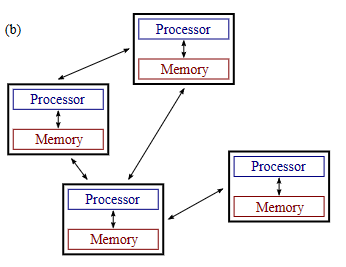
\includegraphics[width=\linewidth]{Distributed System - Wikipedia}
    \caption{System Rozproszony}
    \label{fig:distibutedSystemWikipedia}
    \source{Wikipedia}
\end{figure}

\par W takich systemach komunikacja odbywa się poprzez wymianę wiadomości. Pozwala to na realizację określonych celów. Proces ten może odbywać się z użyciem wielu metod, na przykład z wykorzystaniem protokołu \texttt{HTTP}. Innym rozwiązaniem pozwalającym na wymianę informacji jest wykorzystanie \emph{Message Broker}a.

\subsection{Message Broker i Service Bus}

\par \emph{Message Broker} jest oprogramowaniem, które pełni funkcję pośrednika w komunikacji pomiędzy poszczególnymi aplikacjami. Jest on centralnym punktem odpowiadającym za odbierania, a następnie przesyłanie wiadomości do stron zainteresowanych. Często znajdziemy tutaj rozwiązania, które zapewnią prawidłowe przekazywanie wiadomości według wybranej polityki, możliwość próby ponownego dostarczenia wiadomości, jak i możliwość stworzenia tak zwanej kolejki wiadomości martwych\english{Dead-letter Queue}.

\par Kluczowymi funkcjami \emph{Message Broker}a są:
\begin{itemize}
    \item \emph{Decoupling} - aplikacje komunikują się poprzez centralny punkt, którym jest \emph{Message Broker}, co pozwala im być niezależnymi od siebie. W systemie można dowolnie dodawać, jak i usuwać serwisy, bez negatywnego wpływu na pozostałe serwisy.
    \item \emph{Routing} - pozwala na kierowanie wiadomości na podstawie pewnych ustalonych cech, takich jak na przykład: temat, priorytet lub adresat.
    \item \emph{Reliability} - niezawodność poprzez zapewnienie gwarancji dostarczenia wiadomości, nawet pomimo tymczasowej niedostępności odbiorcy.
    \item Skalowalność\english{Scalability} - możliwość skalowania przepustowości poprzez dodanie kolejnych instancji \emph{Message Broker}a lub przez zastosowanie klastrów.
    \item Bezpieczeństwo - \emph{Message Broker} może oferować uwierzytelnianie i autoryzację, tylko dla klientów posiadających odpowiednie uprawnienia.
    \item Komunikacja asynchroniczna - umożliwia aplikacjom korzystającym z \emph{Message Broker}a dalszą pracę, bez konieczności oczekiwania na odpowiedź.
\end{itemize}

\par \emph{Service Bus} jest bardziej zaawansowanym rozwiązaniem, które oprócz funkcji \emph{Message Brokera} oferuje pełniejsze wsparcie dla transakcji i złożonych operacji. Wchodzi ono zazwyczaj w skład kompleksowych rozwiązań takich jak na przykład \emph{Enterprise Service Bus}. Zapewniają one nie tylko przesyłanie wiadomości, ale i ich koordynację i zarządzanie w ramach skomplikowanych procesów biznesowych.

\begin{figure}
    \centering
    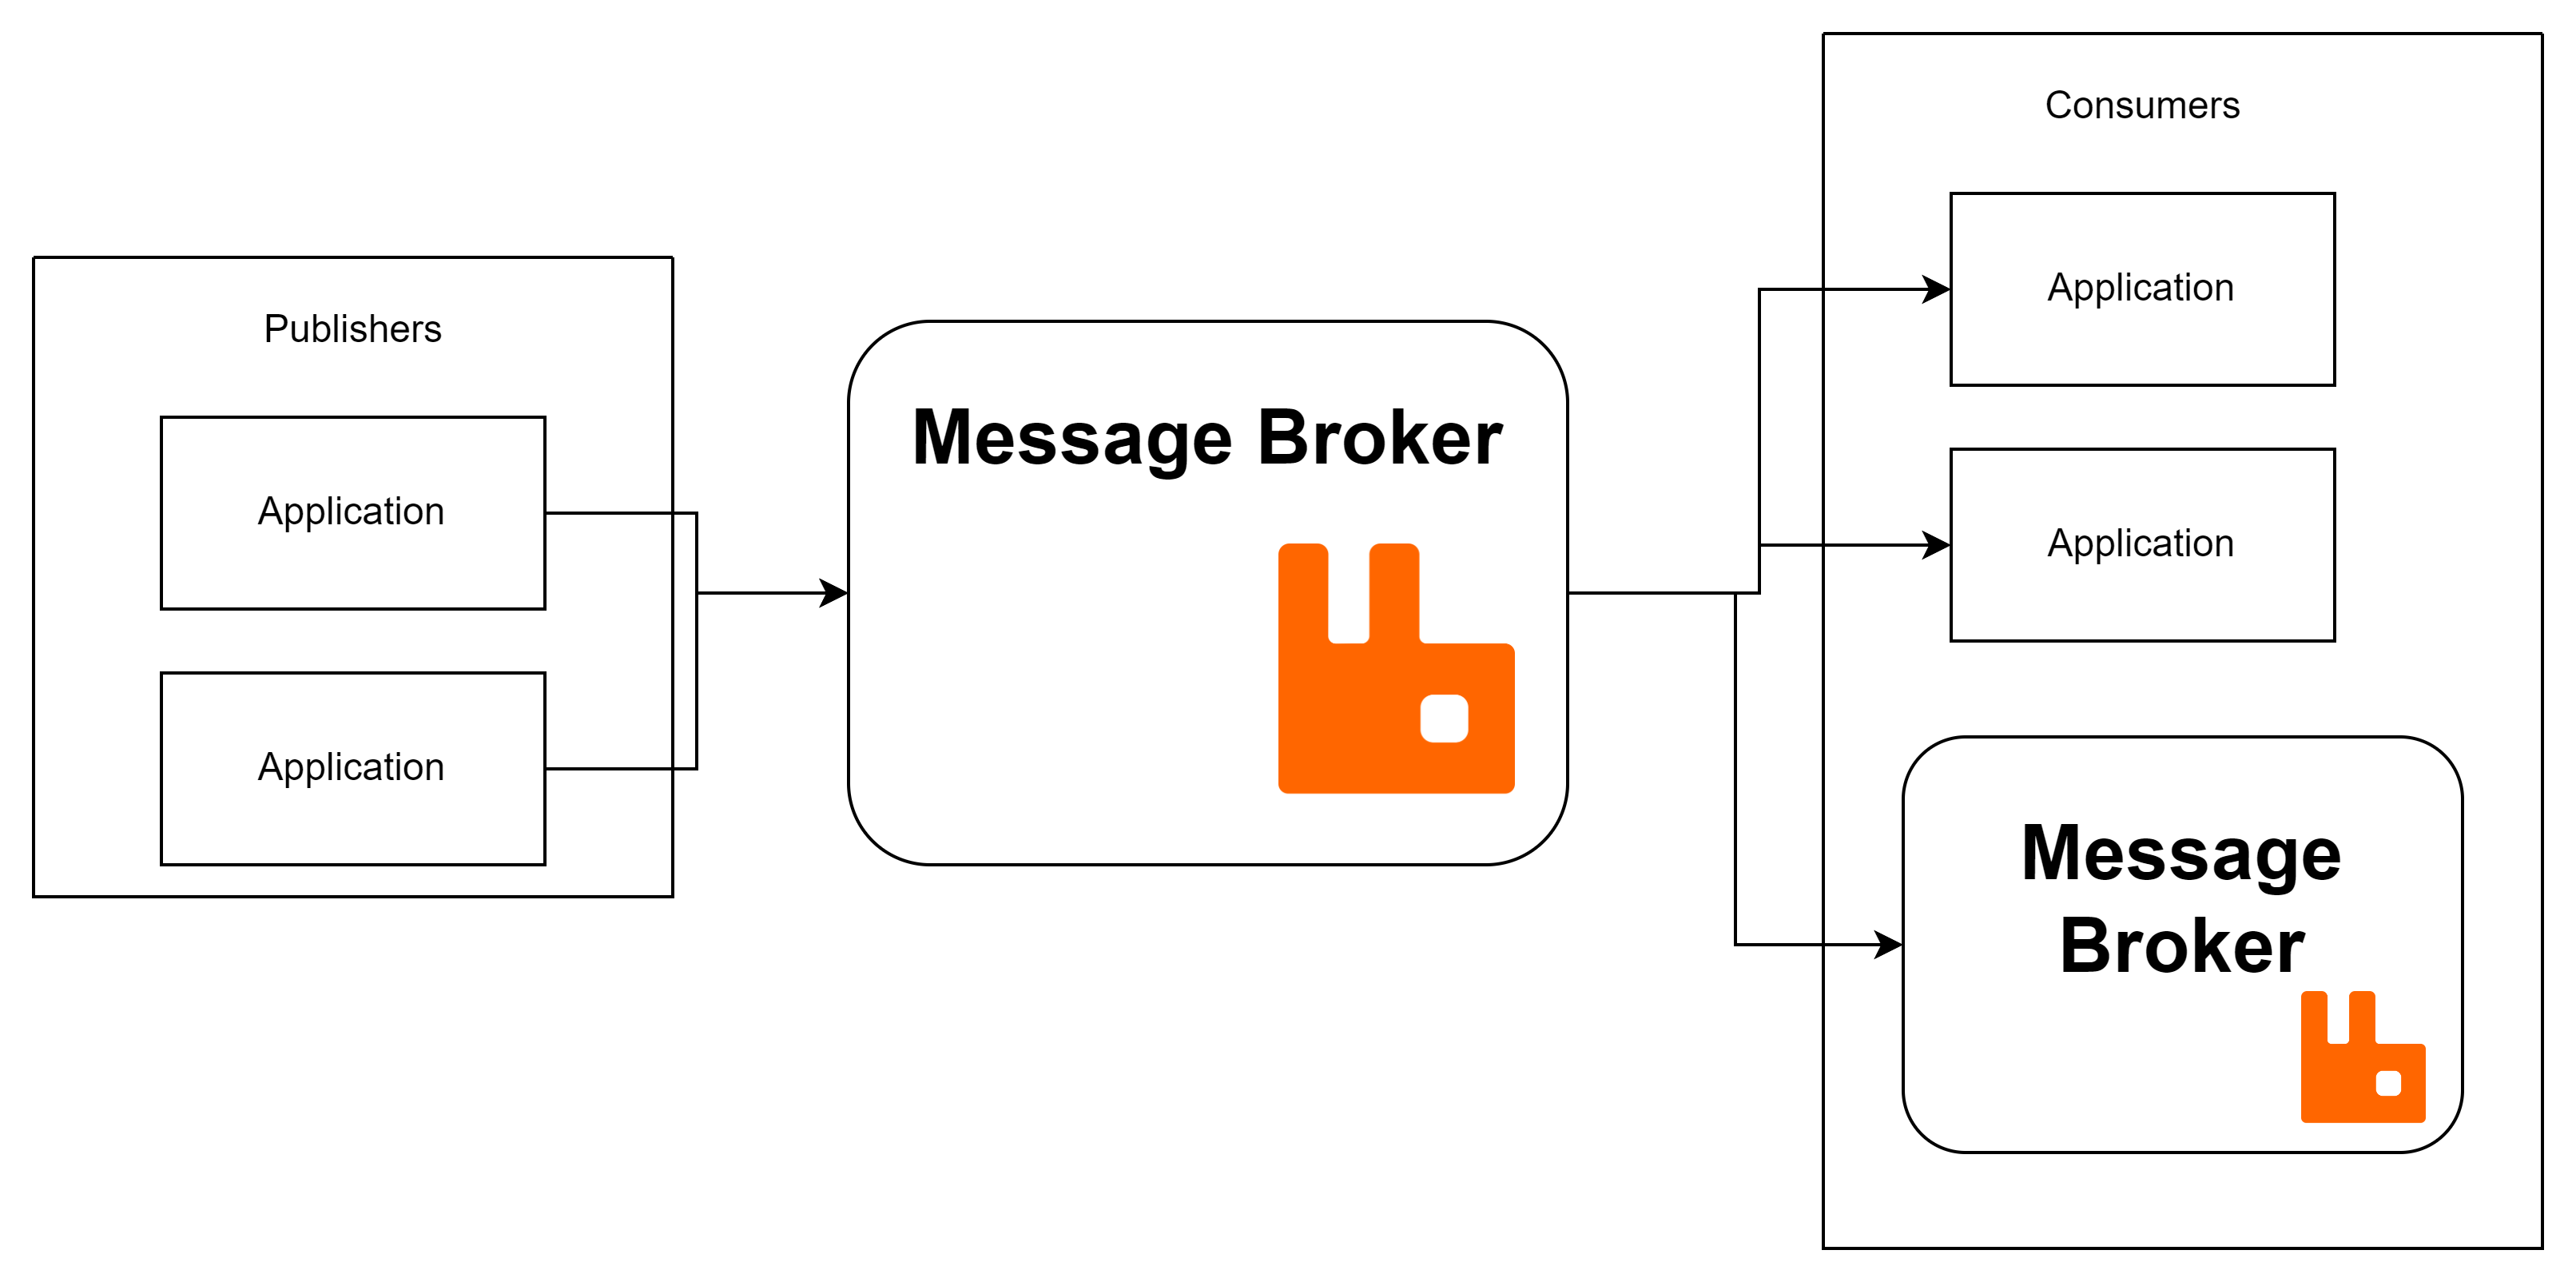
\includegraphics[width=\linewidth]{Service Bus Architecture}
    \caption{Service Bus Architecture}
    \label{fig:serviceBusArchitecture}
    \source{Opracowanie własne}
\end{figure}

\par Przykładami popularnych \emph{Message Broker}ów są: \emph{RabbitMQ}, \emph{Apache Kafka}, \emph{ActiveMQ}, \emph{AWS SNS/SQS} i \emph{Azure Service Bus}.
\section{Przetwarzanie i wykorzystywanie danych geograficznych - OpenStreet Maps}
\section{Symulowanie jednostek w mieście}
\chapter{Implementacja}
\section{Architektura mikroserwisowa}

\par Wykorzystanie architektury mikroserwisowej zapewnia wiele pozytywnych cech, takich jak: 
\begin{itemize}
    \item modularność,
    \item decentralizację,
    \item skalowalność,
    \item oraz zastępowalność i ulepszalność.
\end{itemize}
Jednak stworzenie złożonego systemu rozproszonego, wymaga odpowiedniego podziału odpowiedzialności, jak i znacząco utrudnia monitorowanie i \emph{debug}owanie.

\par Biorąc pod uwagę domenę naszego systemu jesteśmy w stanie wyodrębnić podstawowe zadania oraz oddelegować je do poszczególnych mikroserwisów. W naszym systemie występują: \emph{Message Broker}, \emph{Logger Service}, \emph{API}, \emph{HQ Service}, \emph{Decision System Service} oraz patrole.

% TODO Dopisać bazę danych, jeżeli takowa się pojawi

\par Główną odpowiedzialnością \emph{Message Broker}a w systemie jest centralizacja przesyłu informacji oraz zarządzanie nimi. W tym celu wybrano \emph{RabbitMQ}, który posiada szereg cech przemawiających na jego korzyść. Warto wymienić jego wysoką dostępność, niezawodność, skalowalność oraz elastyczność. \emph{RabbitMQ} obsługuje wiele protokołów komunikacyjnych, takich jak \texttt{AMQP}, \texttt{MQTT} i \texttt{STOMP}, co sprawia, że jest wszechstronnym narzędziem. Dodatkowo oferuje funkcje, takie jak potwierdzanie wiadomości, wzorce \emph{routing}u oraz obsługę opóźnionych wiadomości. Na podstawie badania przeprowadzonego przez \emph{CloudAMQP}\cite{CLOUDAMQP_RABBITMQ_BENCHMARK}, \emph{RabbitMQ} jest w stanie przetworzyć ponad 40 000 wiadomości na sekundę, co świadczy o jego wydajności i przydatności w ramach realizacji tego systemu. Więcej szczegółów dotyczących komunikacji między mikroserwisami można znelźć w podrozdziale \ref{sec:infrastrukturaKomunikacyjna}.

\par Głównymi obowiązkami \emph{HQ Service}u są odbieranie zgłoszeń incydentów występujących w mieście oraz zarządzanie patrolami poprzez monitorowanie ich stanów i wydawanie odpowiednich rozkazów. Ten serwis zawiera także informacje na temat obecnego stanu miasta i promuje wszystkie zdarzenia domenowe\english{Domain Event}, jako odpowiednio zmapowane wydarzenia integracyjne\english{Integration Event}, aby ogłosić zmianę stanu systemu dla pozostałych zainteresowanych serwisów. Więcej na ten temat opisane jest w podrozdziale \ref{sec:infrastrukturaKomunikacyjna}. Tutaj znajduje się \emph{HQ Agent}, odpowiedzialny za zarządzanie i komunikację z agentami patroli (\ref{sec:implementacjaAgentow}).

% TODO Czy generuje raporty?

\par \emph{API} w tym systemie nie pełni aktywnej roli, ale działa w sposób pasywny. Jego głównym zadaniem jest obserwacja zmian i gromadzenie danych. Stanowi ono \emph{back end} dla interfejsu użytkownika, co oznacza, że działa w roli serwera, udostępniając dane dla aplikacji klienckiej. Umożliwia generowanie raportów opartych na zbieranych informacjach, które są agregowane z wydarzeń występujących w systemie. Ponadto, pozwala na prezentację obecnego stanu systemu, co jest istotne dla monitorowania i podejmowania decyzji.

%TODO Decision System Service

\par \emph{Logger Service} ma za zadanie agregować logi z systemu, a do tego celu wykorzystuje \emph{Grafana Loki}\cite{GRAFANA_LOKI_SITE}. Jest to system do zarządzania logami, stworzony przez \emph{Grafana Labs}. Wybór tego narzędzia był podyktowany kilkoma czynnikami, w tym otwartą licencją \texttt{AGPLv3}, łatwością wdrażania w kontenerach \emph{Docker}\cite{DOCKER_SITE} oraz integracją z platformą \emph{Grafana}\cite{GRAFANA_SITE}. \emph{Grafana} zapewnia rozwiązania do monitorowania i wizualizacji danych przechowywanych w Loki. System ten wyróżnia się wysoką skalowalnością oraz prostotą w filtrowaniu otrzymywanych komunikatów, co czyni go efektywnym narzędziem do zarządzania logami w systemie.

\par Każdy patrol składa się z trzech typów mikroserwisów, które komunikują się ze sobą: \emph{Navigation Service}, \emph{Gun Service} i \emph{Patrol Service}. \emph{Patrol Service} pełni rolę punktu centralnego, który integruje pozostałe serwisy. W jego wnętrzu znajduje się agent patrolu, który zakłada funkcjonowanie w radiowozie jako komputer pokładowy.

\par \emph{Navigation Service} jest odpowiedzialny za obsługę nawigacji \emph{GPS}. Serwis ten działa na urządzeniu nawigacyjnym i jest w stanie określić obecną pozycję oraz prowadzić nawigację do wybranego punktu. W skład \emph{Navigation Service} wchodzi \emph{Navigation Agent}, który nadaje otrzymane ze środowiska informacje o obecnej pozycji.

\par Z kolei \emph{Gun Service} to prosty serwis, którego celem jest informowanie innych serwisów o wystrzałach z danego pistoletu. Za przekazywanie tej informacji dalej odpowiada \emph{Gun Agent}. Szczegółowe opisy tych agentów można znaleźć w podrozdziale \ref{sec:implementacjaAgentow}.

\par W aplikacji, ze względu na dużą współdzieloną funkcjonalność między wieloma mikroserwisami, zastosowano wydzielenie tych funkcjonalności do osobnych bibliotek. Architektura aplikacji opiera się na podziale na trzy główne warstwy: wykonawczą (nazywaną w kodzie \emph{Service}), infrastruktury\english{Infrastructure} oraz aplikacji\english{Application}. Każda z tych warstw może zawierać logikę specyficzną dla danego serwisu, ale także posiada swój odpowiednik w wersji współdzielonej\english{Shared}, w której znajdują się fragmenty kodu wykorzystywane przez wszystkie serwisy. Dla przykładu, figura \ref{fig:architectureSharedCodeExample} przedstawia diagram zależności infrastruktury znajdującej się w \emph{HQ Service} i w \emph{Patrol Service}. Dodatkowo istnieje warstwa symulacji, która zawiera implementacje serwisów komunikujących się z symulacją. Dokładniejszy opis tej warstwy znajduje się w podrozdziale \ref{sec:symulacja}.

\begin{figure}
    \centering
    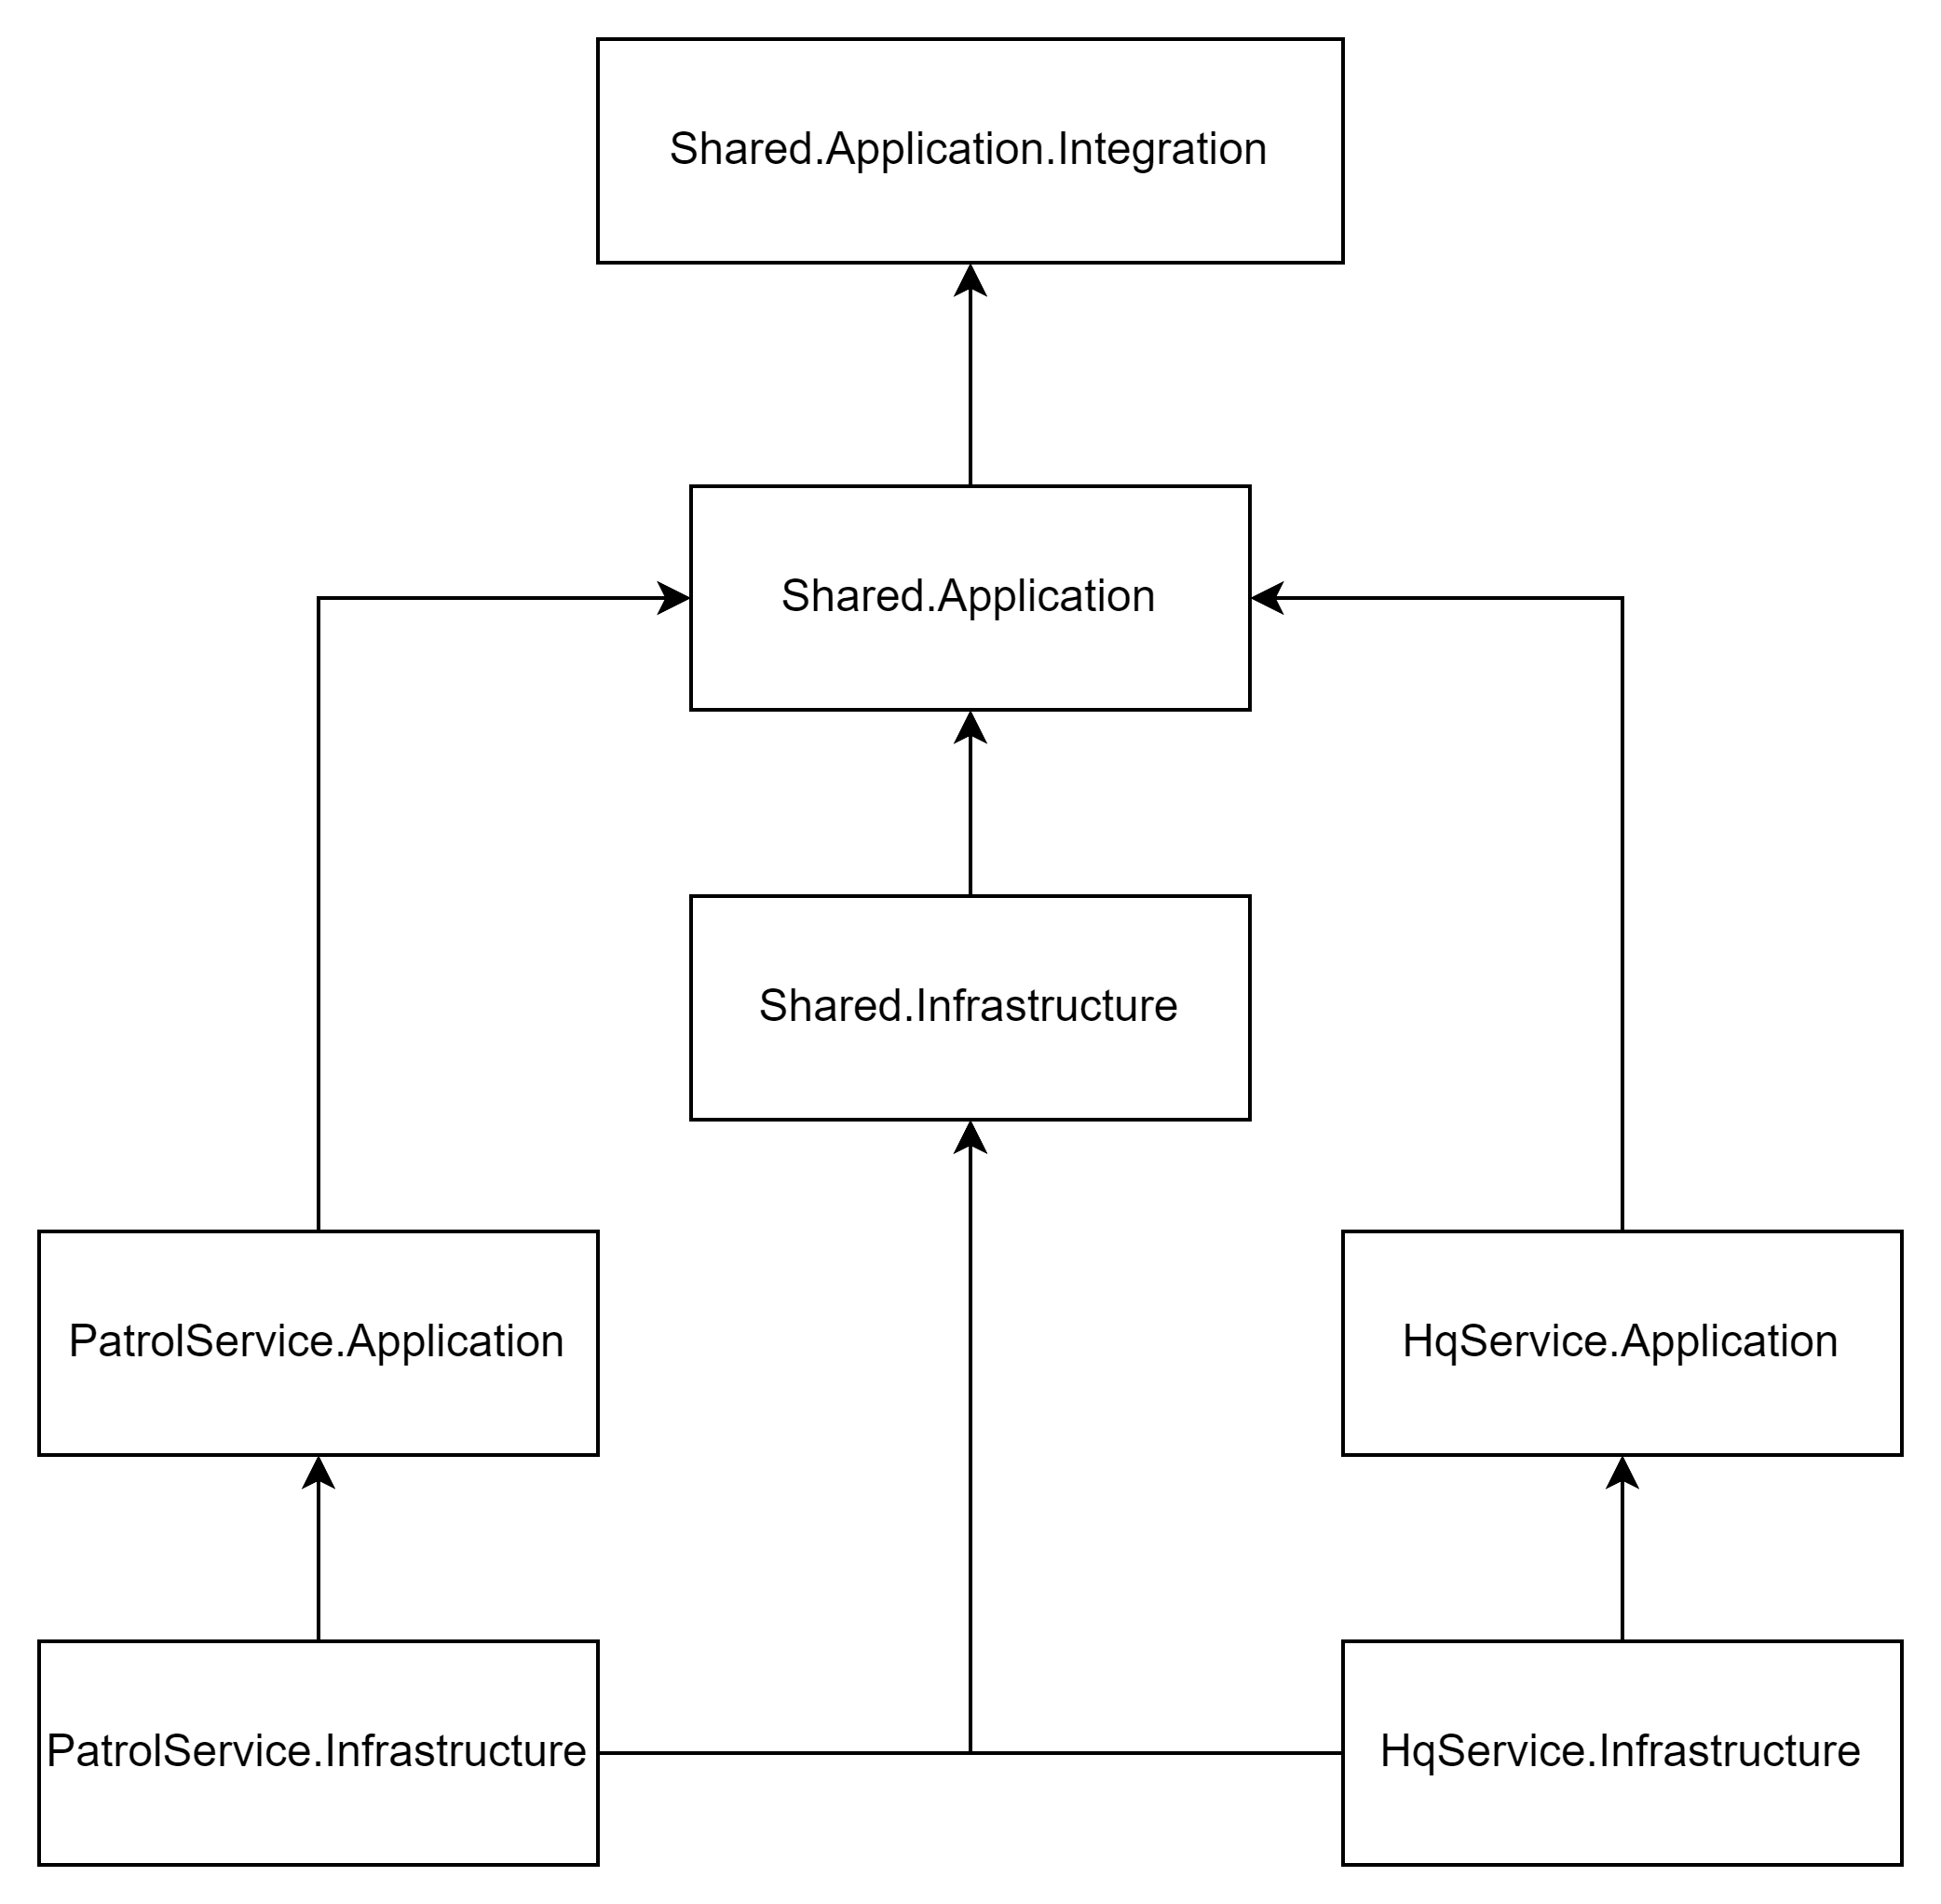
\includegraphics[width=\linewidth]{Architecture - Shared Code - Example}
    \caption{Fragment diagramu zależności przedstawiającego idee współdzielenia kodu pomiędzy serwisami}
    \label{fig:architectureSharedCodeExample}
    \source{Opracowanie Własne}
\end{figure}

\par Warstwa współdzielona zawiera także definicje obiektów domenowych\english{Domain}, bazową implementację agenta oraz wiadomości wysyłane między agentami, które są dokładniej opisane w podrozdziale \ref{sec:implementacjaAgentow}. Dodatkowo, w tej warstwie znajdują się wiadomości integracyjne, które służą do komunikacji między różnymi serwisami. Wyróżniamy trzy rodzaje wiadomości integracyjnych: zdarzenia\english{Event}, zapytania\english{Query} i komendy\english{Command}.

\par Zdarzenia mają za zadanie informować o zmianach w systemie i mogą być odbierane przez dowolną ilość odbiorców. System nie oczekuje żadnej odpowiedzi po publikacji zdarzenia.

\par Zapytania służą do pozyskiwania informacji od innego serwisu. Przewiduje się, że dane zapytanie obsłuży dokładnie jeden odbiorca, który jest wskazany w polu \texttt{Receiver}, i udzieli odpowiedzi w określonym formacie.

\par Komendy służą do wydawania poleceń innemu serwisowi. Mogą mieć tylko jednego odbiorcę, również wskazanego w polu \texttt{Receiver}, i mogą, ale nie muszą, oczekiwać na odpowiedź.

\par Detale dotyczące przesyłania tych wiadomości pomiędzy serwisami opisuje podrozdział \ref{sec:infrastrukturaKomunikacyjna}.

\par Biorąc pod uwagę wszystkie te dane rysuje się nam złożony, wielowarstwowy, ale jednocześnie bardzo modularny system. Aby lepiej zarządzać zależnościami w kodzie, zastosowana została biblioteka \emph{Autofac}\cite{AUTOFAC_SITE}. Pozwala ona na tworzenie modułów, które dodane do naszej aplikacji, samodzielnie załadują odpowiednie zależności w kodzie.

\par Rysunek \ref{fig:architectureNavigationServiceFullDiagram} przedstawia pełen diagram zależności dla \emph{Navigation Service}. Możemy w nim zaobserwować wszystkie rodzaje warstw. Te zaczynające się od \texttt{NavigationService} są specyficzne dla \emph{Navigation Service}. Warstwy znajdujące się w przestrzeni nazw \texttt{Shared}, posiadają kod wspólny dla wszystkich serwisów. Dodatkowo widoczny jest tutaj projekt \texttt{Simulation.Communication}. Zawiera on definicje wiadomości wysyłanych i odbieranych przez symulację. Więcej na ten temat znajduje się w podrozdziale \ref{sec:symulacja}. Analogicznie wyglądają zależności w pozostałych serwisach.

\begin{figure}
    \centering
    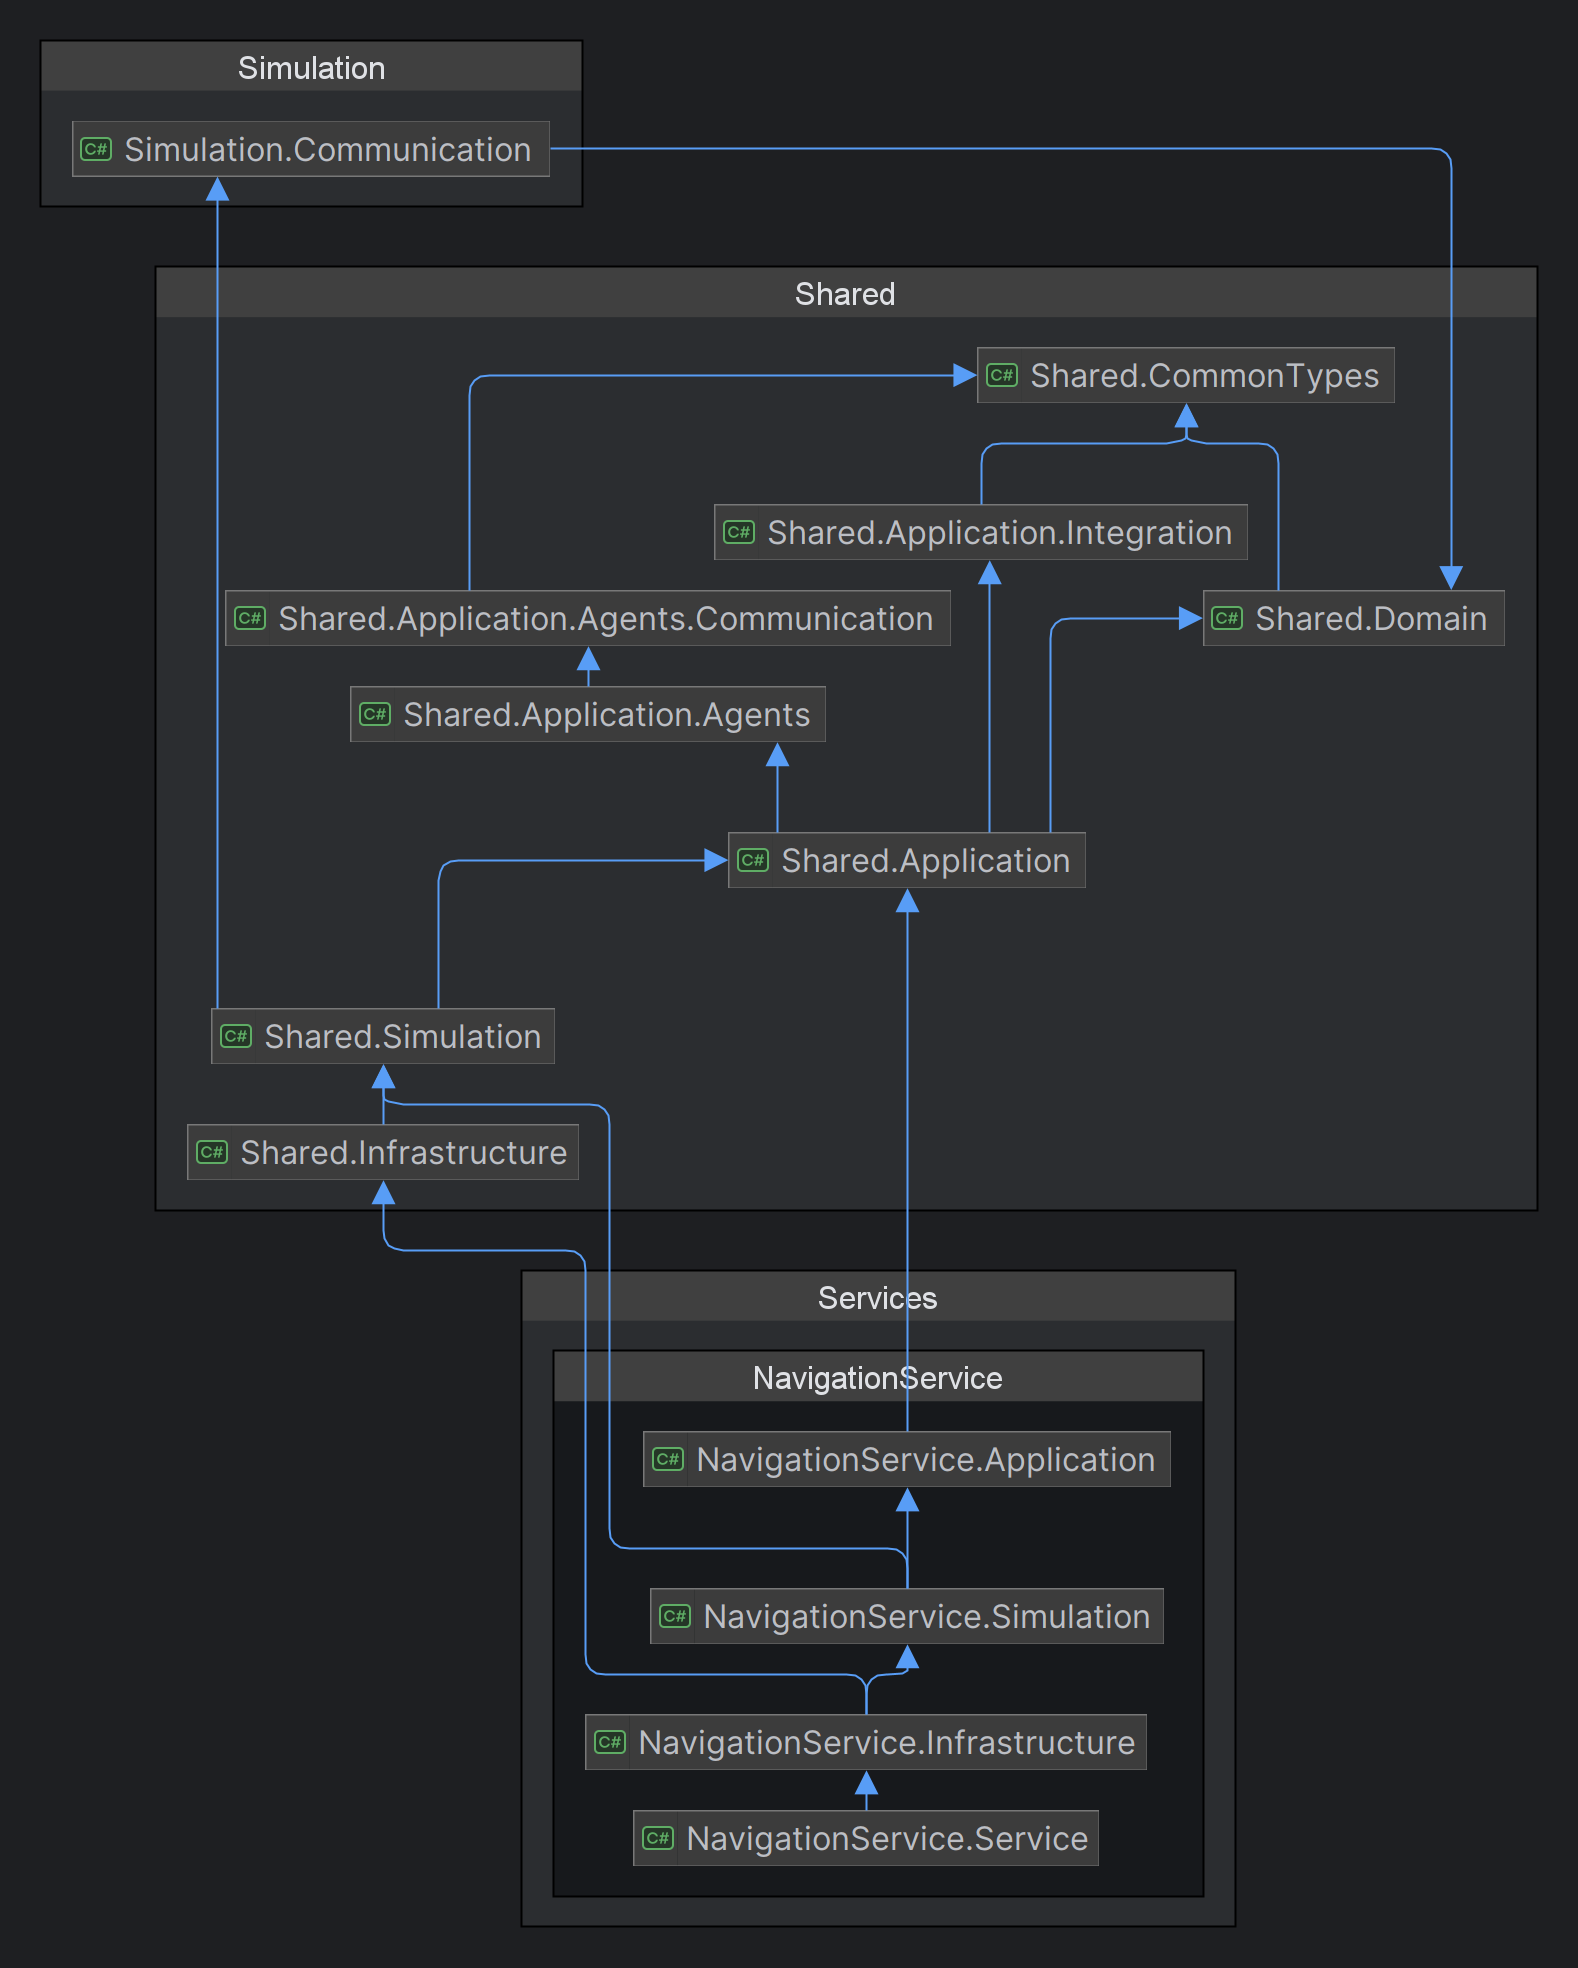
\includegraphics[width=\linewidth]{Architecture - Navigation Service - Full Diagram}
    \caption{Pełen diagram zależności dla \emph{Navigation Service}}
    \label{fig:architectureNavigationServiceFullDiagram}
    \source{Opracowanie Własne}
\end{figure}
\section{Infrastruktura komunikacyjna -- Message Bus i Message Broker}
\label{sec:infrastrukturaKomunikacyjna}

\par Komunikacja w systemie jest oparta na \emph{RabbitMQ}, który pełni funkcję \emph{Message Broker}a. To rozwiązanie umożliwia scentralizowanie całego procesu komunikacji w systemie. W ramach tego rozwiązania różne typy wiadomości (zapytania, wydarzenia i komendy) są przypisane do swoich dedykowanych giełd\english{Exchange}. Poszczególne serwisy subskrybują te giełdy, co pozwala im na odbieranie odpowiednich komunikatów. Wiadomości są serializowane do formatu \texttt{JSON}. Podczas inicjalizacji systemu, automatycznie tworzone są wszystkie kolejki i giełdy wiadomości.

\par W projekcie wykorzystano wzorzec \emph{Message Bus}, który tworzy warstwę abstrakcji dla komunikacji. Serwisy nie są zobowiązane do świadomości, do którego dokładnie adresata kierują komunikat, aby go dostarczyć, jak i są niezależne od konkretnego \emph{Message Broker}a. Jest to zadaniem konkretnej implementacji \texttt{IMessageBus}, aby skierować wiadomości w odpowiednie miejsce. W projekcie skorzystano z implementacji wzorca pochodzącej z \emph{open source}owej biblioteki \emph{parshim/MessageBus}\cite{PARSHIM_MESSAGEBUS_GITHUB}. Wybór tej konkretnej implementacji wynikał z jej zdolności do kierowania wiadomościami nie tylko na podstawie ich typów, ale także ich treści. Była to istotna cecha, biorąc pod uwagę, że w systemie działa wiele kopii tego samego serwisu (na przykład w przypadku patroli), które są w stanie obsłużyć ten sam typ wiadomości. Serwisy korzystające z \emph{Message Broker}a prezentuje grafika \ref{fig:infrastructureServicesRabbitMq}, natomiast na rysunku \ref{fig:infrastructureRabbitMqExchanges} widzimy utworzone przez system giełdy.

\begin{figure}
    \centering
    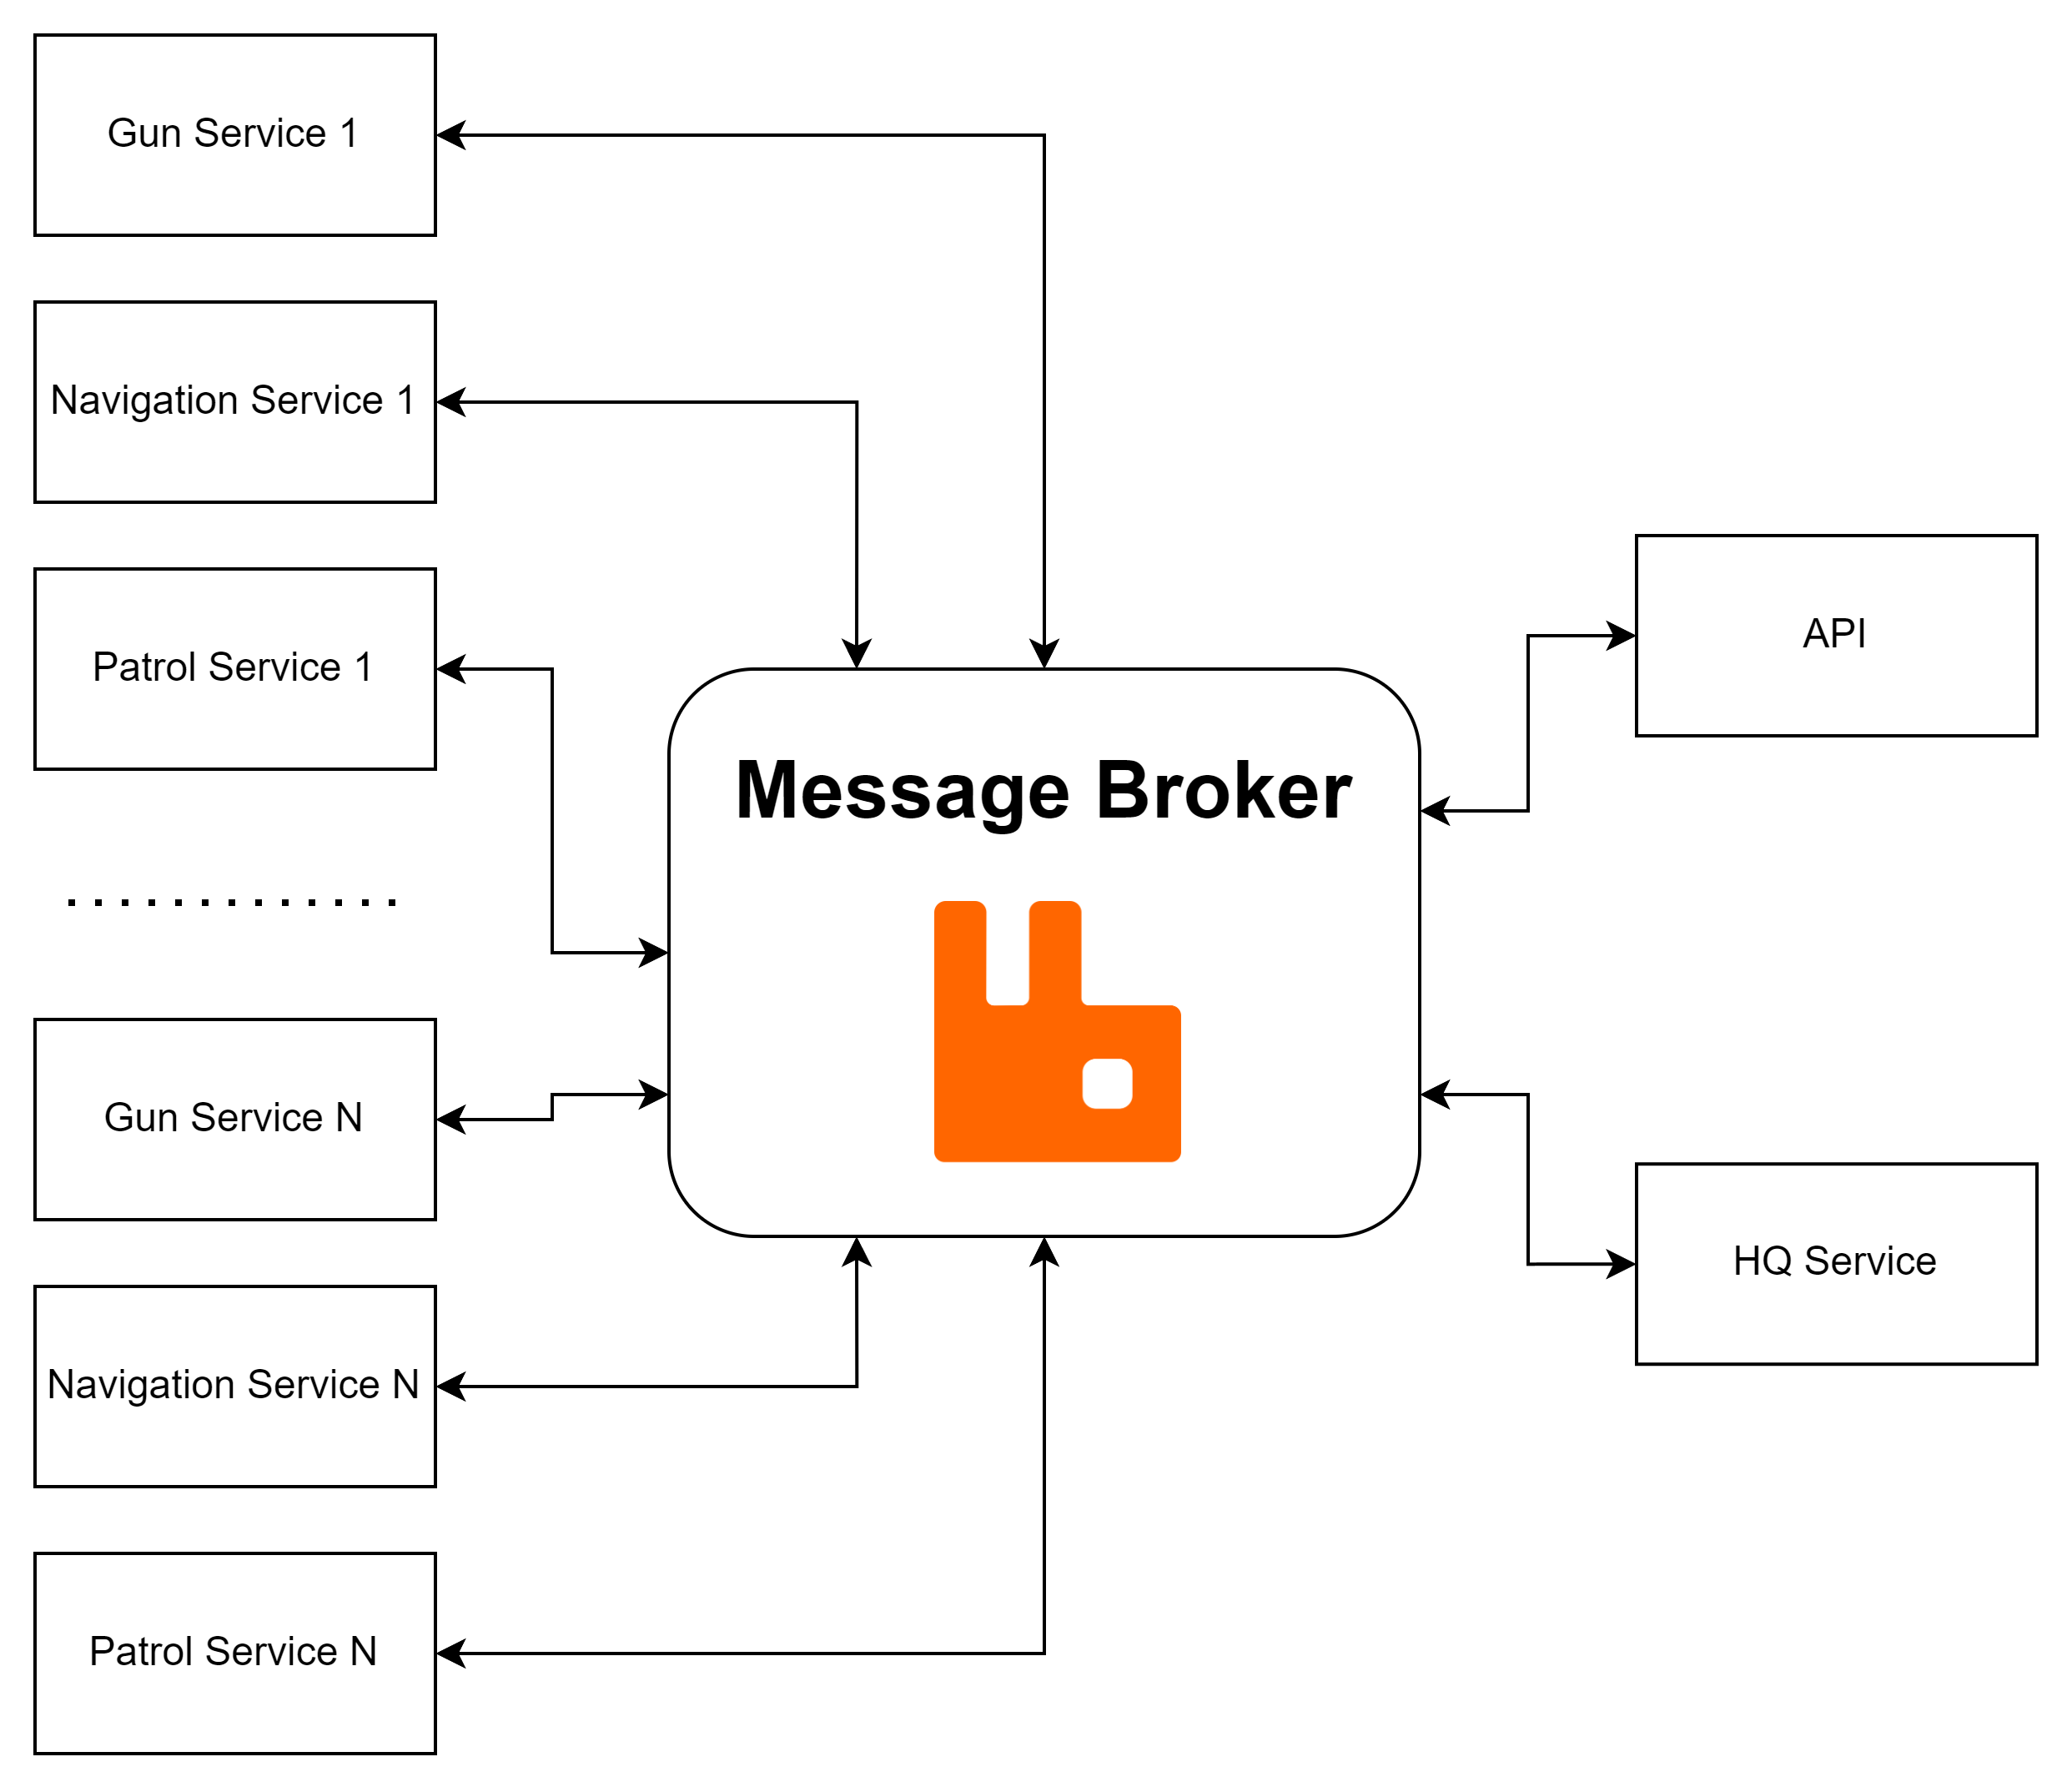
\includegraphics[width=\linewidth]{Infrastructure - Services - RabbitMQ}
    \caption{Diagram przedstawiający serwisy korzystające z \emph{Message Broker}a}
    \label{fig:infrastructureServicesRabbitMq}
    \source{Opracowanie Własne}
\end{figure}

\begin{figure}
    \centering
    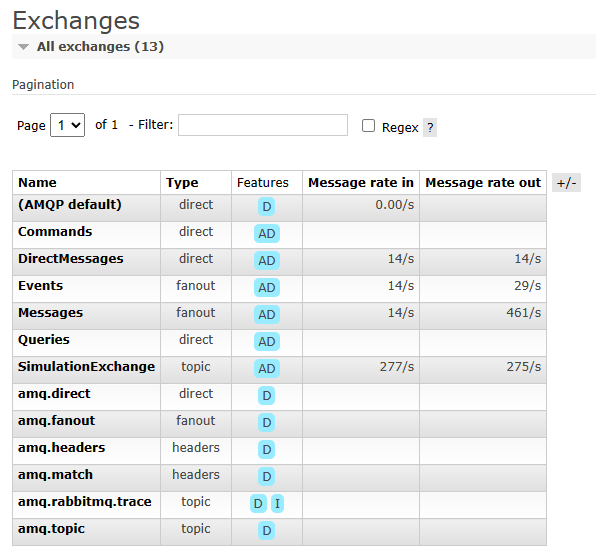
\includegraphics[width=\linewidth]{Infrastructure - RabbitMQ Exchanges}
    \caption{Giełdy w \emph{RabbitMQ} utworzone przez system}
    \label{fig:infrastructureRabbitMqExchanges}
    \source{Opracowanie Własne}
\end{figure}

\par Wiadomości w systemie zostały podzielone na kwerendy\english{Query}, komendy\english{Command} i wydarzenie\english{Event}. Dodatkowo agenci porozumiewają się wiadomościami implementującymi interfejs \texttt{IMessage}, a komunikacja z symulacją odbywa się przy wykorzystaniu komunikatów implementujących \texttt{ISimulationMessage}.

\par Zapytania wysyłane pomiędzy serwisami implementują specjalny interfejs \texttt{IQuery<out TResult>}, który pozwala na wyspecyfikowanie typu oczekiwanego rezultatu. Są wykorzystywane do odpytania innego serwisu w celu uzyskania od niego informacji. System zakłada, że będzie tylko jeden odbiorca takiej wiadomości. Powinien on zostać podany w polu \texttt{Receiver}.

\par Komendy mogą, ale nie muszą zwracać wyniku. Dlatego zostały przygotowane dla nich dwa interfejsy: \texttt{ICommand} i \texttt{ICommand<out TResult>}. Zadaniem tych wiadomości jest wywołanie procesu w innym serwisie, jak i otrzymanie informacji o jego zakończeniu wraz z wynikiem.

\par Zdarzenia w systemie mogą być lokalne lub integracyjne\english{Integration}. To właśnie te drugie, są propagowane w systemie z wykorzystaniem interfejsu \texttt{IEvent}. Ich zadaniem jest poinformowanie o zmianach, jakie zachodzą w systemie. W przypadku zdarzeń, nie oczekuje się na ich rezultat. Są one publikowane w systemie \emph{Fire and Forget}. Odbiorcami są wszystkie serwisy zainteresowane i będące w stanie obsłużyć dane zdarzenie.

\par Wszystkie opisane powyżej typy wiadomości są obsługiwane przez tak zwane \emph{Handler}y, które spełniają jeden z intefejsów: \texttt{IEventHandler<in TEvent>}, \texttt{ICommandHandler<in TCommand, TResult>}, \texttt{ICommandHandler<in TCommand>} lub \texttt{IQueryHandler<in TQuery, TResult>} w zależności od typu danej wiadomości. Klasy spełniające wcześniej wymienione interfejsy są automatycznie znajdywane w danym \texttt{Assembly} i rejestrowane w kontenerze \emph{IoC}\footnote{Inversion of Control}. Rozwiązanie to można porównać do \emph{Event-Driven Architecture}, oczywiście rozszerzonej o komendy i zapytania. Zastosowanie tego rozwiązania pozwoliło w zdecydowanym stopniu zmniejszyć stopień zależności\english{Decoupling} w systemie.

\par Dodatkowo w systemie występują również agenci, ich implementacja została dokładniej omówiona w podrozdziale \ref{sec:implementacjaAgentow}. Komunikacja pomiędzy nimi opiera się na interfejsie \texttt{IMessage}, który został zdefiniowany w taki sposób, aby być otwartym na rozszerzenia i możliwość implementacji własnych mechanizmów opartych o informacje w nim zawarte. Jedną z tych informacji jest pole \texttt{Receivers}, które jest opcjonalne. Jeżeli zawiera ono jaką wartość, to powinna to być lista odbiorców, do których skierowana jest dana wiadomość. W ten sposób \emph{Message Bus} jest w stanie wysłać do nich wiadomość w sposób bezpośredni. Istotnymi są również pola \texttt{MessageId} i \texttt{ResponseTo}, pozwalające na prowadzenie wymiany wiadomości w sposób zorganizowany. Na bazie tych informacji agenci implementują mechanizmy potwierdzania obsłużenia wiadomości i pytania siebie na wzajem o informacje, dokładniej opisane w podrozdziale \ref{sec:implementacjaAgentow}.

\par Symulacja, dokładniej opisana w podrozdziale \ref{sec:symulacja}, również wymaga komunikacji z serwisami działającym w systemie. Odbywa się to przy wykorzystaniu osobnego \emph{Service Bus}a. Możliwym byłoby zastosowanie do tego osobnego \emph{Message Broker}a, jednak tutaj nie zachodziła taka potrzeba, dlatego ta sama instancja \emph{RabbitMQ} obsługuje tę wymianę informacji. Wiadomości spełniające interfejs \texttt{ISimulationMessage} mogą zarówno zostać wysłane przez symulację do danego odbiorcy, jak i zostać do niej nadane, celem poinformowania o podjętej akcji. Dodatkowo został tutaj również wykorzystany mechanizm kwerend, ze względu na konieczność pozyskania informacji o dostępnych dzielnicach\english{District} w mieście przez \emph{HQ Service}.
\section{Implementacja agentów}
\label{sec:implementacjaAgentow} 

\par Agenci stanowią główny trzon decyzyjny systemu. To w nich znajduje się logika odpowiedzialna za podejmowanie decyzji, reagowanie na zmiany i obsługę komunikatów nadawanych przez innych. Podstawowymi założeniami systemów agentowych jest ich autonomiczność, zdolność do komunikacji oraz możliwość postrzegania i wpływania na środowisko. Aby spełnić te wymagania koniecznym były zapewnienie pewnych mechanizmów.

\par Podstawą działania agentów, jest ich umiejętność do postrzegania otoczenia. Odbywa się to przy użyciu \texttt{IEnvironmentSignal}. Każdy agent w systemie definiuje, jakie sygnały z otoczenia potrafi obsłużyć. Następnie serwisy działające w ramach aplikacji, w której żyje nasz agent przekazują mu te sygnały. Trafiają one do specjalnej kolejki, skąd zostaną później obsłużone.

\par Zdolność do działania przejawia się poprzez dostęp do funkcji sprzętowych z poziomu aplikacji. Dla przykładu, \emph{Navigation Agent} potrafi wykorzystać \texttt{INavigationService}, aby ten wyświetlił patrolowi drogę do wyznaczonego celu.

% \par Wszystkie te cechy (sygnały, akcje, wiadomości) można zidentyfikować, jako jedną z tych pięciu kategorii: relacje\english{Relations}, aktywność\english{Activity}, indywidualność\english{Individuality}, czas\english{Time} i lokalizacja\english{Location}. Ich wykaz, miejsce występowania oraz kategoria zostały przedstawione w tabeli \ref{tab:agentsFeaturesCategorization}.

\par Fundamentem podejmowania decyzji przez agentów jest kontekst. Stanowi on zbiór wszystkich cech, które opisują sytuację, w której znajduje się konkretny byt\cite{UNDERSTANDING_AND_USING_CONTEXT} - w naszym przypadku agent. Z powodu istnienia wielu zmiennych należących do kontekstu, systemy na nich oparte potrafią stać się bardzo złożone. W celu efektywnego zarządzania tymi informacjami, można je przypisać do jednej z pięciu kategorii: relacje\english{Relations}, aktywność\english{Activity}, indywidualność\english{Individuality}, czas\english{Time} i lokalizacja\english{Location}\cite{AN_OPERATIONAL_DEFINITION_OF_CONTEXT}. W ramach rozważanego systemu udało się wyodrębnić zmienne kontekstowe, przedstawione w tabeli \ref{tab:agentsFeaturesCategorization}.

\begin{longtable}{|p{0.5\linewidth}|p{0.25\linewidth}|}
    \hline
     Zmienna & Kategoria \\
     \hline
     \hline
     Własna lokalizacja & Lokalizacja \\
     \hline
     Lokalizacja patrolu & Lokalizacja \\
     \hline
     Oczekiwanie na rozkaz & Indywidualność \\
     \hline
     W trakcie patrolowania & Indywidualność \\
     \hline
     W trakcie interwencji & Indywidualność \\
     \hline
     W trakcie strzelaniny & Indywidualność \\
     \hline
     W drodze na strzelaninę & Indywidualność \\
     \hline
     W drodze do interwencji & Indywidualność \\
     \hline
     Rozpoczęcie rozwiązywania incydentu & Aktywność \\
     \hline
     Zakończenie rozwiązywania incydentu & Aktywność \\
     \hline
     Nawigowanie do miejsca docelowego & Aktywność \\
     \hline
     Prezentacja danych dzielnicy & Aktywność \\
     \hline
     Wydanie polecenia patrolowania & Aktywność \\
     \hline
     Wydanie polecenia rozwiązania incydentu & Aktywność \\
     \hline
     Wydanie polecenia wsparcia strzelaniny & Aktywność \\
     \hline
     Wystrzelenie z pistoletu & Indywidualność \\
     \hline
     Stan zarządzanego patrolu & Relacja \\
     \hline
     Stan incydentu & Relacja \\
     \hline
     Stan innego patrolu biorącego udział w strzelaninie & Relacja \\
     \hline
     Czas zgłoszenia incydentu & Czas \\
     \hline
     Czas rozpoczęcia rozwiązywania incydentu & Czas \\
     \hline
      Czas przerodzenia incydentu w strzelaninę & Czas \\
     \hline
      Rozkaz od \emph{HQ} & Relacja \\
     \hline
     Zawiadomienie o incydencie & Relacja \\
     \hline
     Poziom niebezpieczeństwa dzielnicy & Relacja \\
     \hline
\caption{Tabela identyfikacji zmiennych kontekstowych}
\label{tab:agentsFeaturesCategorization}
\end{longtable}

\par Przepływ danych kontekstowych można opisać w postaci ich cyklu życia, zgodnie z regułą \emph{6R}\cite{Klimek2023}. Służy ona do zidentyfikowania zmian zachodzących na zdefiniowanych danych w trakcie ich zbierania\english{Gathering}, \emph{pre-processing}u i \emph{post-processing}u. W ten sposób informacje mogą zostać:
\begin{itemize}
    \item \emph{wyrażone}\english{Represent} - faza zbierania - przechowane w formie niezmienionej,
    \item \emph{rozwiązane}\english{Resolve} - faza zbierania - przekształcone do formy zgodnej z zapotrzebowaniem systemu,
    \item \emph{zachowane}\english{Retain} - faza \emph{pre-processing}u - zapisane w formie niezmienionej względem wyniku poprzedniej fazy,
    \item \emph{wzmocnione}\english{Reinforce} - \emph{pre-processing}u - zgromadzone w ramach większej całości,
    \item \emph{usunięte}\english{Remove} - faza \emph{post-processing}u - takie dane nie są zachowywane, może to być związane na przykład z ich tymczasową przydatnością,
    \item \emph{pozostawione}\english{Remain} - faza \emph{post-processing}u - zachowane do następnej fazy cyklu, czyli do momentu, w którym zostaną nadpisane,
\end{itemize}
W ramach systemu agentowego policji, przepływy te zostały przedstawione w postaci tabeli \ref{tab:r6CycleForContextData}. Został tam również zaznaczony wpływ danego agenta na zmienną kontekstową w postaci operacji: \textbf{read} i \textbf{write}. Gdzie \textbf{read} oznacza, że dany agent jest zainteresowany wartością lecz jej nie modyfikuje, a \textbf{write} oznacza, że dany agent wpływa na tę wartość.

\begin{landscape}
    \begin{longtable}{|p{0.18\linewidth}|p{0.18\linewidth}|p{0.18\linewidth}|p{0.18\linewidth}|p{0.18\linewidth}|}
    \hline
    Zmienna & \emph{Gathering} & \emph{Pre-processing} & \emph{Post-processing} & Agenci zarządzający informacją \\
    \hline
    \hline

     Własna lokalizacja & \textbf{Represent}; Dane pozostają w niezmienionej formie. & \textbf{Reinforce}; Oznaczenie lokalizacji znacznikiem czasowym. & \textbf{Remain}; Iformacja zostaje zachowana, dopóki nie zostanie pobrana jej nowsza wersja.  & \emph{Navigation Agent} (\textbf{read}) jest odpowiedzialny za przetwarzanie danych geograficznych, następnie jest przekazana do \emph{Patrol Agent} (\textbf{read}), który z kolei przesyła ją do \emph{HQ Agent} (\textbf{write}) w postaci \emph{lokalizacji patrolu}. \\
     \hline
     Lokalizacja patrolu & \textbf{Resolve}; Porównanie z posiadanymi już danymi, poprzez weryfikację znacznika czasowego. & \textbf{Reinforce}; Informacja zostaje zachowana jako historia pozycji patrolu. & \textbf{Remain}; Informacja zostaje zapisana. & \emph{HQ Agent} (\textbf{write}) otrzymuje lokalizację patrolu, którą może wykorzystać w procesie decyzyjnym. \\
     \hline
     Oczekiwanie na rozkaz & \textbf{Represent}; Dane pozostają w niezmienionej formie. & \textbf{Reinforce}; Stan wzbogacany o znacznik czasowy. & \textbf{Remain}; Informacja zostaje zapisana. & \emph{Patrol Agent} (\textbf{write}) aktualizuje swój stan. Jest on przekazywany do \emph{HQ Agent} (\textbf{read}) w postaci \emph{stanu zarządzanego patrolu}. \\
     \hline
     W trakcie patrolowania & \textbf{Represent}; Dane pozostają w niezmienionej formie. & \textbf{Reinforce}; Stan wzbogacany o znacznik czasowy. & \textbf{Remain}; Informacja zostaje zapisana. & \emph{Patrol Agent} (\textbf{write}) aktualizuje swój stan. Jest on przekazywany do \emph{HQ Agent}(\textbf{read}) w postaci \emph{stanu zarządzanego patrolu}. \\
     \hline
     W trakcie interwencji & \textbf{Represent}; Dane pozostają w niezmienionej formie. & \textbf{Reinforce}; Stan wzbogacany o znacznik czasowy. & \textbf{Remain}; Informacja zostaje zapisana. & \emph{Patrol Agent} (\textbf{write}) aktualizuje swój stan. Jest on przekazywany do \emph{HQ Agent} (\textbf{read}) w postaci \emph{stanu zarządzanego patrolu}. \\
     \hline
     W trakcie strzelaniny & \textbf{Represent}; Dane pozostają w niezmienionej formie. & \textbf{Reinforce}; Stan wzbogacany o znacznik czasowy. & \textbf{Remain}; Informacja zostaje zapisana. & \emph{Patrol Agent} (\textbf{write}) aktualizuje swój stan. Jest on przekazywany do \emph{HQ Agent} (\textbf{read}) w postaci \emph{stanu zarządzanego patrolu}. \\
     \hline
     W drodze na strzelaninę & \textbf{Represent}; Dane pozostają w niezmienionej formie. & \textbf{Reinforce}; Stan wzbogacany o znacznik czasowy. & \textbf{Remain}; Informacja zostaje zapisana. & \emph{Patrol Agent} (\textbf{write}) aktualizuje swój stan. Jest on przekazywany do \emph{HQ Agent} (\textbf{read}) w postaci \emph{stanu zarządzanego patrolu}. \\
     \hline
     W drodze do interwencji & \textbf{Represent}; Dane pozostają w niezmienionej formie. & \textbf{Reinforce}; Stan wzbogacany o znacznik czasowy. & \textbf{Remain}; Informacja zostaje zapisana. & \emph{Patrol Agent} (\textbf{write}) aktualizuje swój stan. Jest on przekazywany do \emph{HQ Agent} (\textbf{read}) w postaci \emph{stanu zarządzanego patrolu}. \\
     \hline
     Nawigowanie do miejsca docelowego & \textbf{Represent}; Dane pozostają w niezmienionej formie. & \textbf{Reinforce}; Obliczona zostaje trasa. & \textbf{Remain}; Trasa jest wykorzystywana podczas procesu nawigacji. & \emph{Navigation Agent} (\textbf{write}) wykonuje akcję nawigowania. \\
     \hline
     Prezentacja danych dzielnicy & \textbf{Represent}; Dane pozostają w niezmienionej formie. & \textbf{Reinforce}; Pobrany zostaje obszar dzielnicy. & \textbf{Remain}; Pobrane dane są wyświetlane, aby usprawnić nawigowanie po dzielnicy. & \emph{Navigation Agent} (\textbf{write}) pomaga w procesie patrolowania dzielnicy. \\
     \hline
     Wydanie polecenia patrolowania & \textbf{Represent}; Dane pozostają w niezmienionej formie. & \textbf{Retain}; Dane pozostają w niezmienionej formie.  & \textbf{Remove}; Rozkaz zostaje wysłany, nie jest on później wykorzystywany\footnote{\label{note:ZapisanieStanuPatrolu}Dopiero zmiana stanu, jaka nastąpi w patrolu, zostanie zachowana jako zaobserwowany stan systemu.}. & \emph{HQ Agent} (\textbf{write}) wydaje polecenie patrolowania patrolowi. Jest ono odbierane przez \emph{Patrol Agent} (\textbf{read}) w postaci \emph{rozkazu od HQ}. \\
     \hline
     Wydanie polecenia rozwiązania incydentu & \textbf{Represent}; Dane pozostają w niezmienionej formie. & \textbf{Retain}; Dane pozostają w niezmienionej formie. & \textbf{Remove}; Rozkaz zostaje wysłany, nie jest on później wykorzystywany\footref{note:ZapisanieStanuPatrolu}. & \emph{HQ Agent} (\textbf{write}) wydaje polecenie rozwiązania incydentu patrolowi. Jest ono odbierane przez \emph{Patrol Agent} (\textbf{read}) w postaci \emph{rozkazu od HQ}. \\
     \hline
     Wydanie polecenia wsparcia strzelaniny & \textbf{Represent}; Dane pozostają w niezmienionej formie. & \textbf{Retain}; Dane pozostają w niezmienionej formie. & \textbf{Remove}; Rozkaz zostaje wysłany, nie jest on później wykorzystywany\footref{note:ZapisanieStanuPatrolu}. & \emph{HQ Agent} (\textbf{write}) wydaje polecenie wsparcia strzelaniny patrolowi. Jest ono odbierane przez \emph{Patrol Agent} (\textbf{read}) w postaci \emph{rozkazu od HQ}. \\
     \hline
     Wystrzelenie z pistoletu & \textbf{Represent}; Dane pozostają w niezmienionej formie. & \textbf{Reinforce}; Dane zostają wzbogacone o znacznik czasowy i dane incydentu. & \textbf{Remain}; Informacja zostaje zgłoszona do \emph{HQ Agent} w postaci zmiany stanu zdarzenia.  & \emph{Gun Agent} (\textbf{read}) obserwuje wystrzał z pistoletu, następnie przekazuje tę informację do \emph{Patrol Agent} (\textbf{write}), który wzbogaca ją o kontekst. \\
     \hline
     Stan zarządzanego patrolu & \textbf{Resolve}; Dane zostają odfiltrowana na podstawie ich aktualności i obecnego stanu wiedzy. & \textbf{Reinforce}; Informacja zostaje dodana do kolekcji stanów patrolu. Może wywołać zmianę stanu incydentu. & \textbf{Remain}; Informacja zostaje zachowana w historii. & \emph{HQ Agent} (\textbf{read}) otrzymuje informację o zmianie stanu patrolu. \\
     \hline
     Stan incydentu & \textbf{Resolve}; Dane zostają odfiltrowana na podstawie ich aktualności i obecnego stanu wiedzy. & \textbf{Reinforce}; Informacja zostaje dodana do kolekcji stanów incydentu. & \textbf{Remain}; Informacja zostaje zachowana. & \emph{Patrol Agent} (\textbf{write}) wysyła do \emph{HQ Agent} (\textbf{read}) informację o zmianie stanu incydentu. \\
     \hline
     Stan innego patrolu biorącego udział w strzelaninie & \textbf{Resolve}; Dane zostają odfiltrowana na podstawie ich aktualności i obecnego stanu wiedzy. & \textbf{Retain}; Dane pozostają w niezmienionej formie. & \textbf{Remain}; Informacja zostaje zachowana. & \emph{Patrol Agent} (\textbf{read}) obserwuje zmianę stanu innego patrolu, poprzez jego dołączenie do strzelaniny. \\
     \hline
     Czas zgłoszenia incydentu & \textbf{Represent}; Dane pozostają w niezmienionej formie. & \textbf{Reinforce}; Informacja zostaje dodana jako wpis do historii przebiegu incydentu. & \textbf{Remain}; Informacja zostaje zachowana. & \emph{HQ Agent} (\textbf{read}) otrzymuje informację o nowym incydencie. \\
     \hline
     Czas rozpoczęcia rozwiązywania incydentu & \textbf{Represent}; Dane pozostają w niezmienionej formie. & \textbf{Reinforce}; Informacja zostaje dodana jako wpis do historii przebiegu incydentu. & \textbf{Remain}; Informacja zostaje zachowana. & \emph{HQ Agent} (\textbf{read}) obserwuje zmianę stanu incydentu i na jej podstawie dokonuje wpisu. \\
     \hline
     Czas przerodzenia incydentu w strzelaninę & \textbf{Represent}; Dane pozostają w niezmienionej formie. & \textbf{Reinforce}; Informacja zostaje dodana jako wpis do historii przebiegu incydentu. & \textbf{Remain}; Informacja zostaje zachowana. & \emph{HQ Agent} (\textbf{read}) obserwuje zmianę stanu incydentu i na jej podstawie dokonuje wpisu. \\
     \hline
     Rozkaz od \emph{HQ}  & \textbf{Resolve}; Dane zostają odfiltrowana na podstawie ich aktualności i obecnego stanu wiedzy. & \textbf{Reinforce}; Informacja zostaje skojarzona z dzielnicą miasta. Dodatkowo zostaje odpowiednio zinterpretowana. & \textbf{Remain}; Rozkaz zostaje zachowany. & \emph{Patrol Agent} (\textbf{read}) otrzymuje rozkaz. \\
     \hline
     Zawiadomienie o incydencie  & \textbf{Resolve}; Informacja zostaje odfiltrowana na bazie obecnego stanu wiedzy, aby uniknąć duplikatów. & \textbf{Reinforce}; Informacje o incydencie zostają skojarzone z dzielnicą i jej poziomem niebezpieczeństwa. & \textbf{Remain}; Informacja zostaje zapisana. & \emph{HQ Agent} (\textbf{read}) otrzymuje zgłoszenie nowego incydentu. \\
     \hline
      Poziom niebezpieczeństwa danej dzielnicy &  \textbf{Represent}; Dane pozostają w niezmienionej formie. & \textbf{Reinforce}; Dane zostają skojarzone z incydentami i lokalizacjami patroli. & \textbf{Remain}; Informacja zostaje zachowana. & \emph{HQ Agent} (\textbf{read}) otrzymuje informację o poziomie niebezpieczeństwa dzielnicy. \\
      \hline
    \caption{Cykl \emph{R6} dla zmiennych kontekstowych}
    \label{tab:r6CycleForContextData}
    \end{longtable}
\end{landscape}


% \par Dodatkowo, w systemie można opisać cykl życia zmiennych kontekstowych w następujący sposób:
% \begin{itemize}
%     \item Lokalizacja - jest pobierana przez \emph{Navigation Agent}, następnie przekazywana do \emph{Patrol Agent}, który przekazuje ją do \emph{HQ Agent}. Ten decyduje o tym, czy posiada już nowszą wersję tej informacji, czy też nie. W zależności od tego ignoruje lub zachowuje daną informację. Dodatkowo informacja ta jest wzbogacana o kontekst związany z dzielnicą.
%     \item Trasa do celu - jest pobierana przez \emph{Nabigation Agent}, który następnie zachowuje ją u siebie i wyświetla.
%     \item Wystrzał - sygnał obserwowany przez \emph{Gun Agent}, następnie przekazywany do \emph{Patrol Agent} i kierowany dalej do \emph{HQ Agent}, który na jej podstawie ogłasza alarm i wysyła jednostki w ramach wsparcia.
%     \item Rozpoczęcie interwencji - sygnał obserwowany przez \emph{Patrol Agent}, zachowywany i przekazywany do \emph{HQ Agent}.
%     \item Zakończenie interwencji - sygnał obserwowany przez \emph{Patrol Agent}, zachowywany i przekazywany do \emph{HQ Agent}.
%     \item Zakończenie strzelaniny - sygnał obserwowany przez \emph{Patrol Agent}, zachowywany i przekazywany do \emph{HQ Agent}. Jednostka główna musi zdecydować, czy komunikat, który otrzymała nie jest duplikatem, jako iż, w strzelaninie może brać więcej niż jeden patrol.
%     \item Poziom niebezpieczeństwa dzielnicy - informacja na ten temat jest posiadana przez \emph{HQ Agent}, na podstawie której wydaje on rozkazy patrolowania i rozwiązywania incydentów.
% \end{itemize}

\par Komunikacja między agentami odbywa się przy wykorzystaniu \emph{Message Bus}a, opisanego w podrozdziale \ref{sec:infrastrukturaKomunikacyjna}. Wszystkie wiadomości spełniają interfejs \texttt{IMessage}, a agenci definiują które ich typy są w stanie obsłużyć. Oczywiście sama możliwość wysłania komunikatu, nie rozwiązuje wszystkich problemów w dialogu, dlatego też zostały zaimplementowane dwa dodatkowe mechanizmy rozszerzające bazowe możliwości.

\par Pierwszym z nich jest możliwość odpytania\english{Ask} innego agenta i oczekiwania na odpowiedź. Jest to niezbędny mechanizm, podczas podejmowania decyzji wymagających danych, których dany agent nie posiada.

\par Drugim wysyłanie wiadomości wymagających potwierdzenia odbioru\english{Requiring Acknowledgment}. Dla nich powstał specjalny interfejs \texttt{IMessageWithAcknowledgeRequired} rozszerzający \texttt{IMessage}. Mechanizm ten jest wykorzystywany podczas wysyłania rozkazów przez \emph{HQ Agent}, aby mieć pewność ich akceptacji.

\par Podstawowe założenia agenta w systemie definiuje interfejs \texttt{IAgent}. Określa on konieczność zdefiniowania akceptowanych typów sygnałów środowiskowych i akceptowanych typów wiadomości. Klasa \texttt{AgentBase} jest bazową implementacją rozszerzającą tę definicję o wspomniane wcześniej mechanizmy potwierdzania wiadomości i odpytywania innych agentów.

\par Agenci spełniają dodatkowo \texttt{IHostedService}, co pozwala na uruchomienie ich, jako długo działające\english{Long Running} programy\cite{BACKGROUND_TASKS_WITH_HOSTED_SERVICES}. Ich działanie jest w pełni asynchroniczne. Dzięki zastosowaniu mechanizmu dostępu warunkowego, w postaci \texttt{AsyncReaderWriterLock} pochodzącego z biblioteki \emph{AsyncEx}\cite{STEPHEN_CLEARY_ASYNCEX_GITHUB}, mogą oni odczytywać wiadomości, które trafiły do kolejek. Cykl działania agenta przedstawia rysunek \ref{fig:agentsAgentCycle}.

\begin{figure}
    \centering
    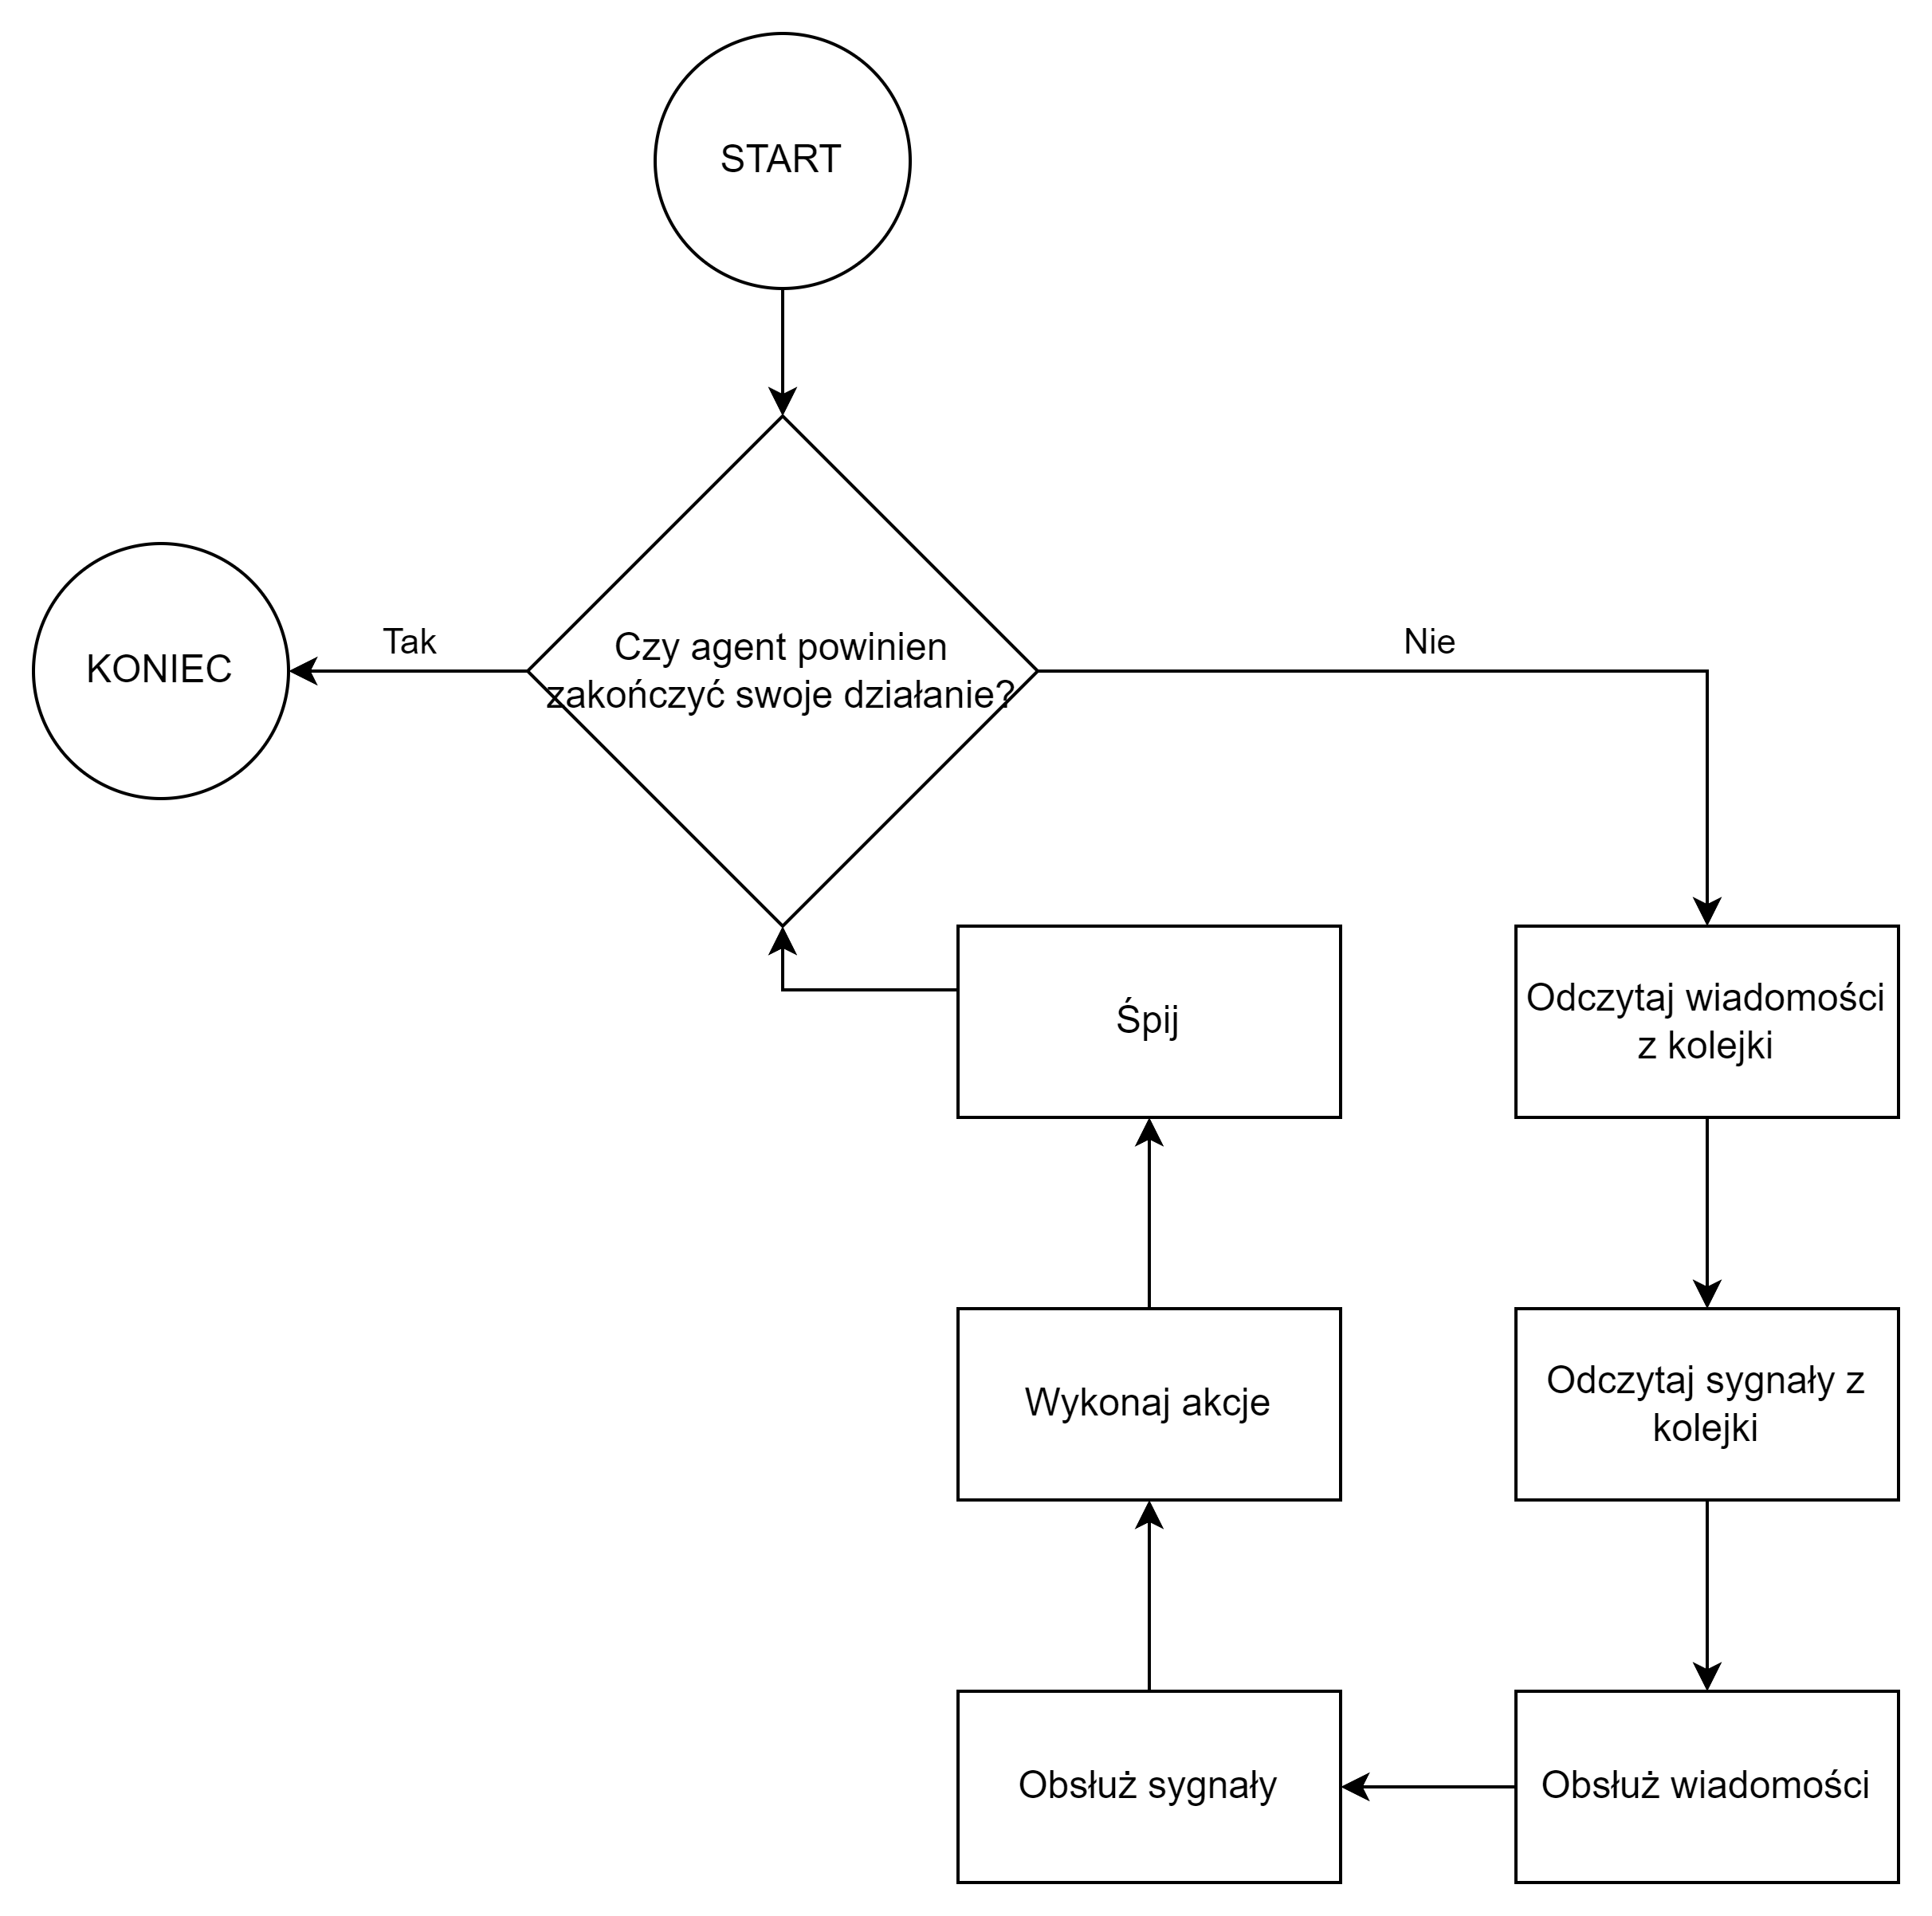
\includegraphics[width=\linewidth]{Agents - Agent Cycle}
    \caption{Cykl działania agenta}
    \label{fig:agentsAgentCycle}
    \source{Opracowanie Własne}
\end{figure}

\par Aby spełnić założenia systemu, ważnym było dokładne określenie wymiany wiadomości między agentami. Tabela \ref{tab:agentsMessagesSenderReceiver} pokazuje relację między typem wiadomości, a jej odbiorcą i nadawcą.

\begin{table}
    \centering
    \begin{tabular}{|c|c|c|} 
     \hline
     Rodzaj wiadomości & Nadawca & Odbiorca \\
     \hline
     \hline
     AskPositionMessage & Patrol Agent & Navigation Agent \\ 
     \hline
     CurrentLocationMessage & Navigation Agent & Patrol Agent \\ 
     \hline
     CurrentLocationMessage & Patrol Agent & HQ Agent \\ 
     \hline
     DestinationReachedMessage & Navigation Agent & Patrol Agent \\ 
     \hline
     GunFiredMessage & Gun Agent & Patrol Agent \\ 
     \hline
     GunFiredMessage & Patrol Agent & HQ Agent \\ 
     \hline
     IncidentInvestigationStartedMessage & Patrol Agent & HQ Agent \\ 
     \hline
     IncidentResolvedMessage & Patrol Agent & HQ Agent \\ 
     \hline
     JoinedShootingMessage & Patrol Agent & HQ Agent \\ 
     \hline
     NavigateToMessage & Patrol Agent & Navigation Agent \\ 
     \hline
     PatrolOfflineMessage & Patrol Agent & HQ Agent \\ 
     \hline
     PatrolOnlineMessage & Patrol Agent & HQ Agent \\ 
     \hline
     PatrolStatusChangedMessage & Patrol Agent & HQ Agent \\ 
     \hline
     ShowDistrictMessage & Patrol Agent & Navigation Agent \\ 
     \hline
     HandleIncidentOrderMessage & HQ Agent & Patrol Agent \\ 
     \hline
     PatrolDistrictOrderMessage & HQ Agent & Patrol Agent \\ 
     \hline
     SupportShootingOrderMessage & HQ Agent & Patrol Agent \\ 
     \hline
    \end{tabular}
    \caption{Tabela relacji wiadomości, nadawcy i odbiorcy}
    \label{tab:agentsMessagesSenderReceiver}
\end{table}

\par Zdefiniowane został również sygnały środowiskowe, służące agentom do obserwowania zmian w ich otoczeniu. Przedstawia je tabela \ref{tab:agentsEnvironmentSignals}.

\begin{table}
    \centering
    \begin{tabular}{|c|c|} 
     \hline
     Rodzaj sygnału & Agent \\
     \hline
     \hline
     DestinationReachedSignal & Navigation Agent \\ 
     \hline
     GunFiredSignal & Gun Agent \\ 
     \hline
     IncidentAlreadyOverSignal & Patrol Agent \\ 
     \hline
     IncidentResolvedSignal & Patrol Agent \\ 
     \hline
     PositionChangedSignal & Navigation Agent \\ 
     \hline
    \end{tabular}
    \caption{Tabela sygnałów środowiskowych wraz z ich odbiorcami}
    \label{tab:agentsEnvironmentSignals}
\end{table}

\par Aby komunikacja mogła nastąpić pomiędzy agentami, koniecznym jest ich odpowiednia konfiguracja. W szczególności dotyczy to patroli, które muszą wiedzieć, z jakich elementów się składają. W tym celu powstał interfejs \texttt{IPatrolInfoService}, który zapewnia informacje o identyfikatorach \emph{Patrol Agent}, \emph{Navigation Agent} i \emph{Gun Agent} oraz identyfikator patrolu, jako całości. Dokładniejszy opisz konfiguracji został omówiony w podrozdziale \ref{sec:konfiguracja}.
\section{Problemy decyzyjne}
\label{sec:algorytmDecyzyjny}

\par \emph{HQ Agent}, dokładniej opisany w podrozdziale \ref{sec:implementacjaAgentow}, jest odpowiedzialny za podejmowanie decyzji w ramach zarządzania jednostkami patroli w mieście. Jego głównym celem jest podejmowanie decyzji, które będą skutkować w jak największej efektywności działania systemu. Aby określić jego efektywności postanowiono wybrać kilka cech, które pozwolą to stwierdzić. Więcej na ten temat znajduje się w podrozdziale \ref{sec:problemBadawczy}.

\par Miasto jest organizmem, który nieustannie podlega zmianom, dlatego przy podejmowaniu decyzji, nie można brać pod uwagę, tylko i wyłącznie, jego obecnego stanu. Należy również pamiętać o utrzymaniu pewnej rezerwy zasobów, na wypadek zaistnienia nieprzewidzianych sytuacji. Aby rozwiązać ten problem, konieczne jest podjęcie dwóch decyzji. Pierwsza z nich dotyczy rozmieszczenia patroli w poszczególnych dzielnicach, natomiast druga podjętych działań w przypadku zaistnienia incydentów.

\par Aby zbadać wpływ rozmieszczenia patroli w mieście, postanowiono wykorzystać dwie różne metody przydzielania patroli do dzielnic. Pierwsza z nich ma za zadanie przydzielić patrole równomiernie\english{Even distribution}, natomiast druga wykorzystuje wiedzę na temat danych dzielnic i dokonuje decyzji na bazie priorytetów. Zapotrzebowanie danej dzielnicy jest określane na podstawie jej poziomu niebezpieczeństwa. Jest to zmienna konfigurowalna, dokładniej opisana w podrozdziale \ref{sec:konfiguracja}. W pierwszej kolejności zostaną tutaj wybrane rejony, którym najbardziej brakuje jednostek, według ich opisu, we wcześniej wspomnianej konfiguracji.

\par W przypadku zaistnienia incydentu, decyzja zostaje podjęta na podstawie algorytmu wykorzystującego wagi, gdzie każdy z wolnych patroli podlega ocenie. Wybrany zostanie ten patrol, do którego zostanie przypisany najlepszy wynik. Cechy, jakie bierz pod uwagę ten algorytm to:
\begin{itemize}
    \item Dystans - określa odległość, jaką patrol musiałby przebyć, aby dotrzeć na miejsce. Obliczana wartości jest normalizowana, na bazie odległości jakie otrzymały pozostałe patrole, gdzie wartość $0$ otrzyma patrol znajdujący się najdalej, natomiast wartość $1$ patrol najbliższy.
    \item Przypisanie patrolu do dystryktu, w którym dzieje się incydent - $1$, gdy patrol jest przypisany do dzielnicy, w której znajduje się incydent; $0$, gdy patrol jest przypisany do innej dzielnicy.
    \item Czy zabranie patrolu spowoduje deficyt - wartość ta, jest określana na podstawie obecnej liczby patroli w danej dzielnicy, do której przypisany jest rozważany patrol. Jeżeli zmiana ta spowoduje powstanie lub powiększenie się deficytu, wtedy patrol otrzymuje niższy wynik. Wartości są znormalizowane do przedziału $[0,1]$. 
\end{itemize}

\par Ostateczna ocena patrolu jest obliczana na podstawie wzoru:
$$
x = f_1*w_1+f_2*w_2+f_3*w_3
$$
gdzie $f_1$, $f_2$, $f_3$ to wymienione wcześniej cechy, a $w_1$, $w_2$, $w_3$ to wagi. Wpływ na działanie algorytmu ma konfiguracja, opisana dokładniej w podrozdziale \ref{sec:konfiguracja}.

\par Opisany powyżej mechanizm, nie jest stosowany w przypadku wsparcia dla strzelanin. Ponieważ strzelaniny są sytuacjami wyjątkowymi, w sytuacji, w której zdarzy się jej pojawienie, system podejmie decyzję na podstawie odległości i wybierze najbliższy patrol.
\section{Integracja z PostGIS}
\section{Wizualizacja systemu i \emph{API}}

\par Aby umożliwić obserwowanie działania systemu powstała \emph{aplikacja webowa}. Jej głównymi zadaniami jest obserwowanie zmian zachodzących w systemie, aby umożliwić wygenerowanie statystyk dotyczących jego działania, jak i pozwolić na wizualizację bieżącego stanu systemu. Interfejs graficzny, został oparty o technologię \emph{React}\cite{REACT_SITE}, z wykorzystaniem paczek \emph{MobX}\cite{MOBX_SITE} oraz \emph{React Leaflet}\cite{REACT_LEAFLET_SITE}.

\par Stworzony w ten sposób interfejs, pozwala na wyświetlanie bieżących pozycji patroli oraz incydentów, które wystąpiły w systemie. Centralna część pozwala na obserwowanie obecnego stanu mapy, natomiast lista po lewej stronie wyświetla działające w systemie patrole wraz z ich stanem. Możliwe jest ich wybranie, aby zostały one zaznaczone na mapie odmiennym kolorem. Nad tą listą znajduje się panel, który wyświetla obecny stan systemu. Wszystkie te elementy możemy zaobserwować na grafice \ref{fig:uiWhole}.

\begin{figure}
    \centering
    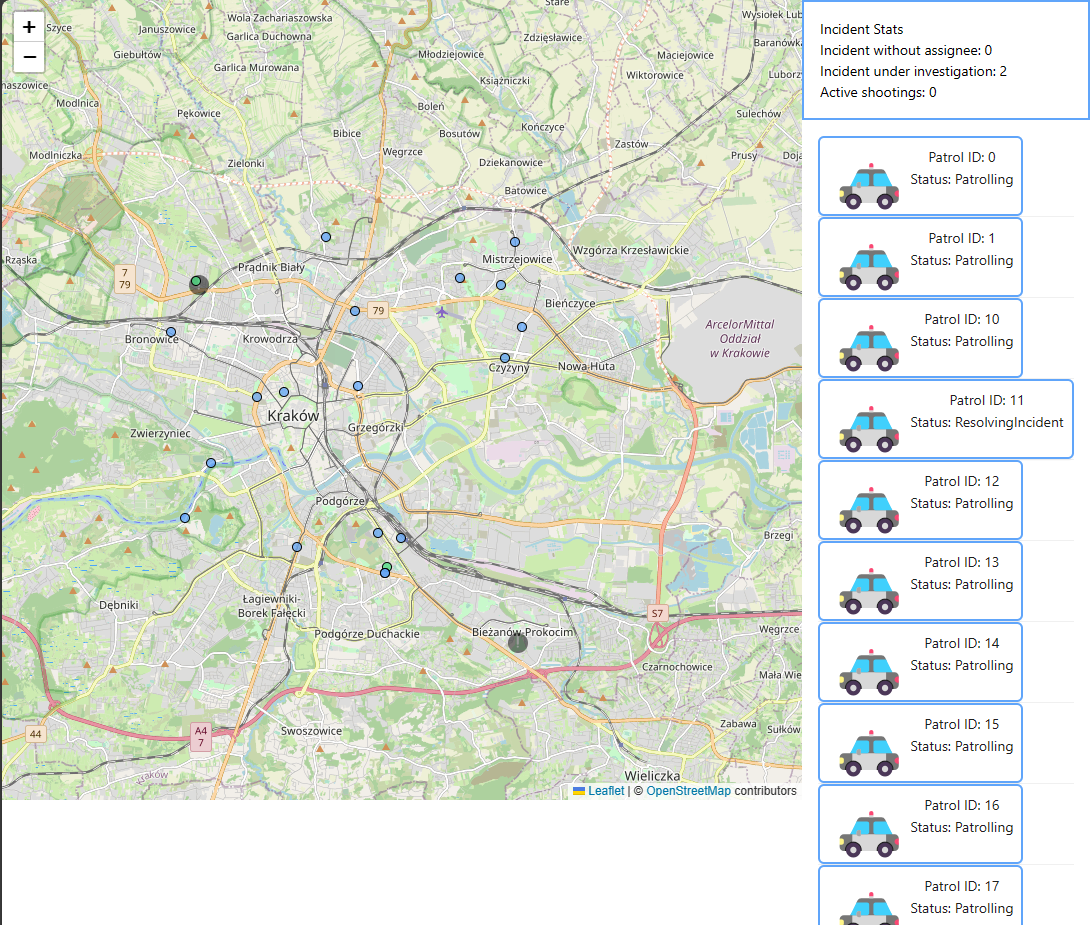
\includegraphics[width=\linewidth]{UI - Whole User Interface}
    \caption{Interfejs użytkownika}
    \label{fig:uiWhole}
    \source{Opracowanie Własne}
\end{figure}

\par Widoczne na mapie znaczniki w kształcie kolorowych kółek, są patrolami. Ich kolor wskazuje na posiadany stan. W systemie wyróżniamy stany:
\begin{itemize}
    \item \emph{Patrolling} - niebieski - oznacza patrol, którego obecnym zadaniem jest patrolowanie wyznaczonego mu obszaru.
    \item \emph{ResolvingIncident} - zielony - oznacza patrol, który został przypisany do konkretnego incydentu.
    \item \emph{InShooting} - czerwony - oznacza patrol, który bierze aktywny udział w strzelaninie lub zmierza, w roli wsparcia, do strzelaniny. W tym stanie prędkość patrolu jest zwiększona i zależy ona od konfiguracji opisanej w podrozdziale \ref{sec:konfiguracja}.
    \item Morski - oznacza patrole, które zostały wybrane, kotrzystając z listy patroli.
\end{itemize}

\par Incydenty zostały oznaczone za pomocą znaczników z wykrzyknikami w środku. Jeżeli wykrzyknik jest czarny, oznacza to, że dane zdarzenie przebiega normalnie. Z kolei, znaczniki posiadające czerwony znak wykrzyknienia, oznaczają strzelaniny.

\begin{figure}
    \centering
    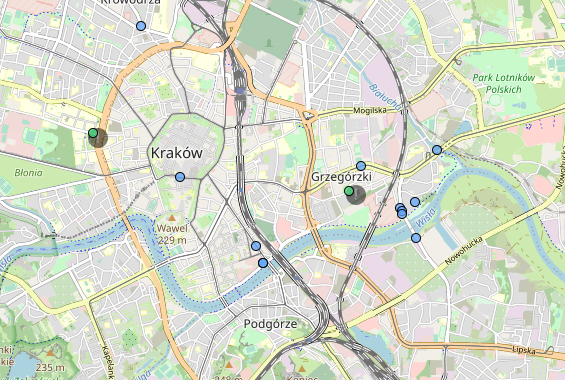
\includegraphics{UI - Patrols - Patrolling and Solving}
    \caption{Patrols - \emph{ResolvingIncident}}
    \label{fig:uiPatrolsPatrollingAndSolving}
    \source{Opracowanie Własne}
\end{figure}

\begin{figure}
    \centering
    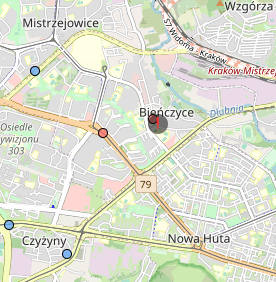
\includegraphics{UI - Patrols - Shooting}
    \caption{Patrols - \emph{InShooting}}
    \label{fig:uiPatrolsInShooting}
    \source{Opracowanie Własne}
\end{figure}

\par Informacje o zmianach, jakie nastąpiły w systemie, wyświetlają się na bieżąco, dzięki zastosowaniu technologii \emph{SignalR}\cite{SIGNALR_SITE}. Dane o nowych incydentach i patrolach, jak i aktualizacje ich stanów i pozycji, są automatycznie wysyłane do podłączonych klientów. Pozwala to na obserwowanie stanu systemu w czasie rzeczywistym.

\par Na podstawie zebranych danych \emph{API} potrafi również wygenerować pliki ze statystykami. Dane zgromadzone w ten sposób, zostały wykorzystane do analizy działania systemu i oceny wpływu informacji kontekstowych na proces decyzyjny. Informacje zawarte w tych plikach to: historia poruszania się patroli, historia stanów patroli, historia przebiegów incydentów, oraz dane wykorzystywane w procesie decyzyjnym, takie jak średnia odległość dostępnych patroli od wybranego incydentu.
\section{Symulacja}
\label{sec:symulacja}

\par Pierwszym wyzwaniem na jakie natrafimy podczas dyskusji o symulacji w systemie rozproszonym jest asynchroniczna\english{Asynchronous} natura zdarzeń, dziejących się w tym systemie. W celu obsłużenia wiadomości, mogących pojawić się w dowolnym momencie, został zaimplementowany specjalny \texttt{IMessageService}, który gromadzi komunikaty, a następnie pozwala na ich odczytanie w dogodnym momencie.

\par Zastosowana implementacja jest symulacją ciągłą. Po każdym wykonaniu pętli logiki, następuje przerwa, której długość jest obliczana według wzoru:

\begin{algorithmic}
\State $cycleDuration = cycleEndTime - cycleStartTime$
\State $delay \gets 1 / 60 - cycleDuration$
\If {$delay \geq 0$}
    \State $finalDelay \gets delay$
\Else 
    \State $finalDelay \gets 0$ 
\EndIf
\end{algorithmic}

Natomiast wszystkie akcje, podczas aktualizacji stanu obiektów symulowanych, biorą pod uwagę ilość czasu, jaka upłynęła od ostatniego kroku. Wartość ta jest odpowiednio skalowana, korzystając z ustawiania \emph{TimeRate}, które pochodzi z konfiguracji. Więcej na ten temat, można doczytać w podrozdziale \ref{sec:konfiguracja}.

\par Diagram \ref{fig:simulationMainLoop} przedstawia przebieg głównej pętali symulacji. Zaznaczeni w nim reżyserowie\english{Director}, to specjalne obiekty, które spełniają interfejs \texttt{IDirector}. Dzięki temu, w razie potrzeby, system można w prosty sposób rozszerzyć o kolejne elementy zarządzające jego stanem. Każdy z nich posiada pewną kompetencję, której zarządzaniem się zajmuje. Obecnie zostały zaimplementowane \texttt{IncidentDirector} i \texttt{PatrolDirector}.

\begin{figure}
    \centering
    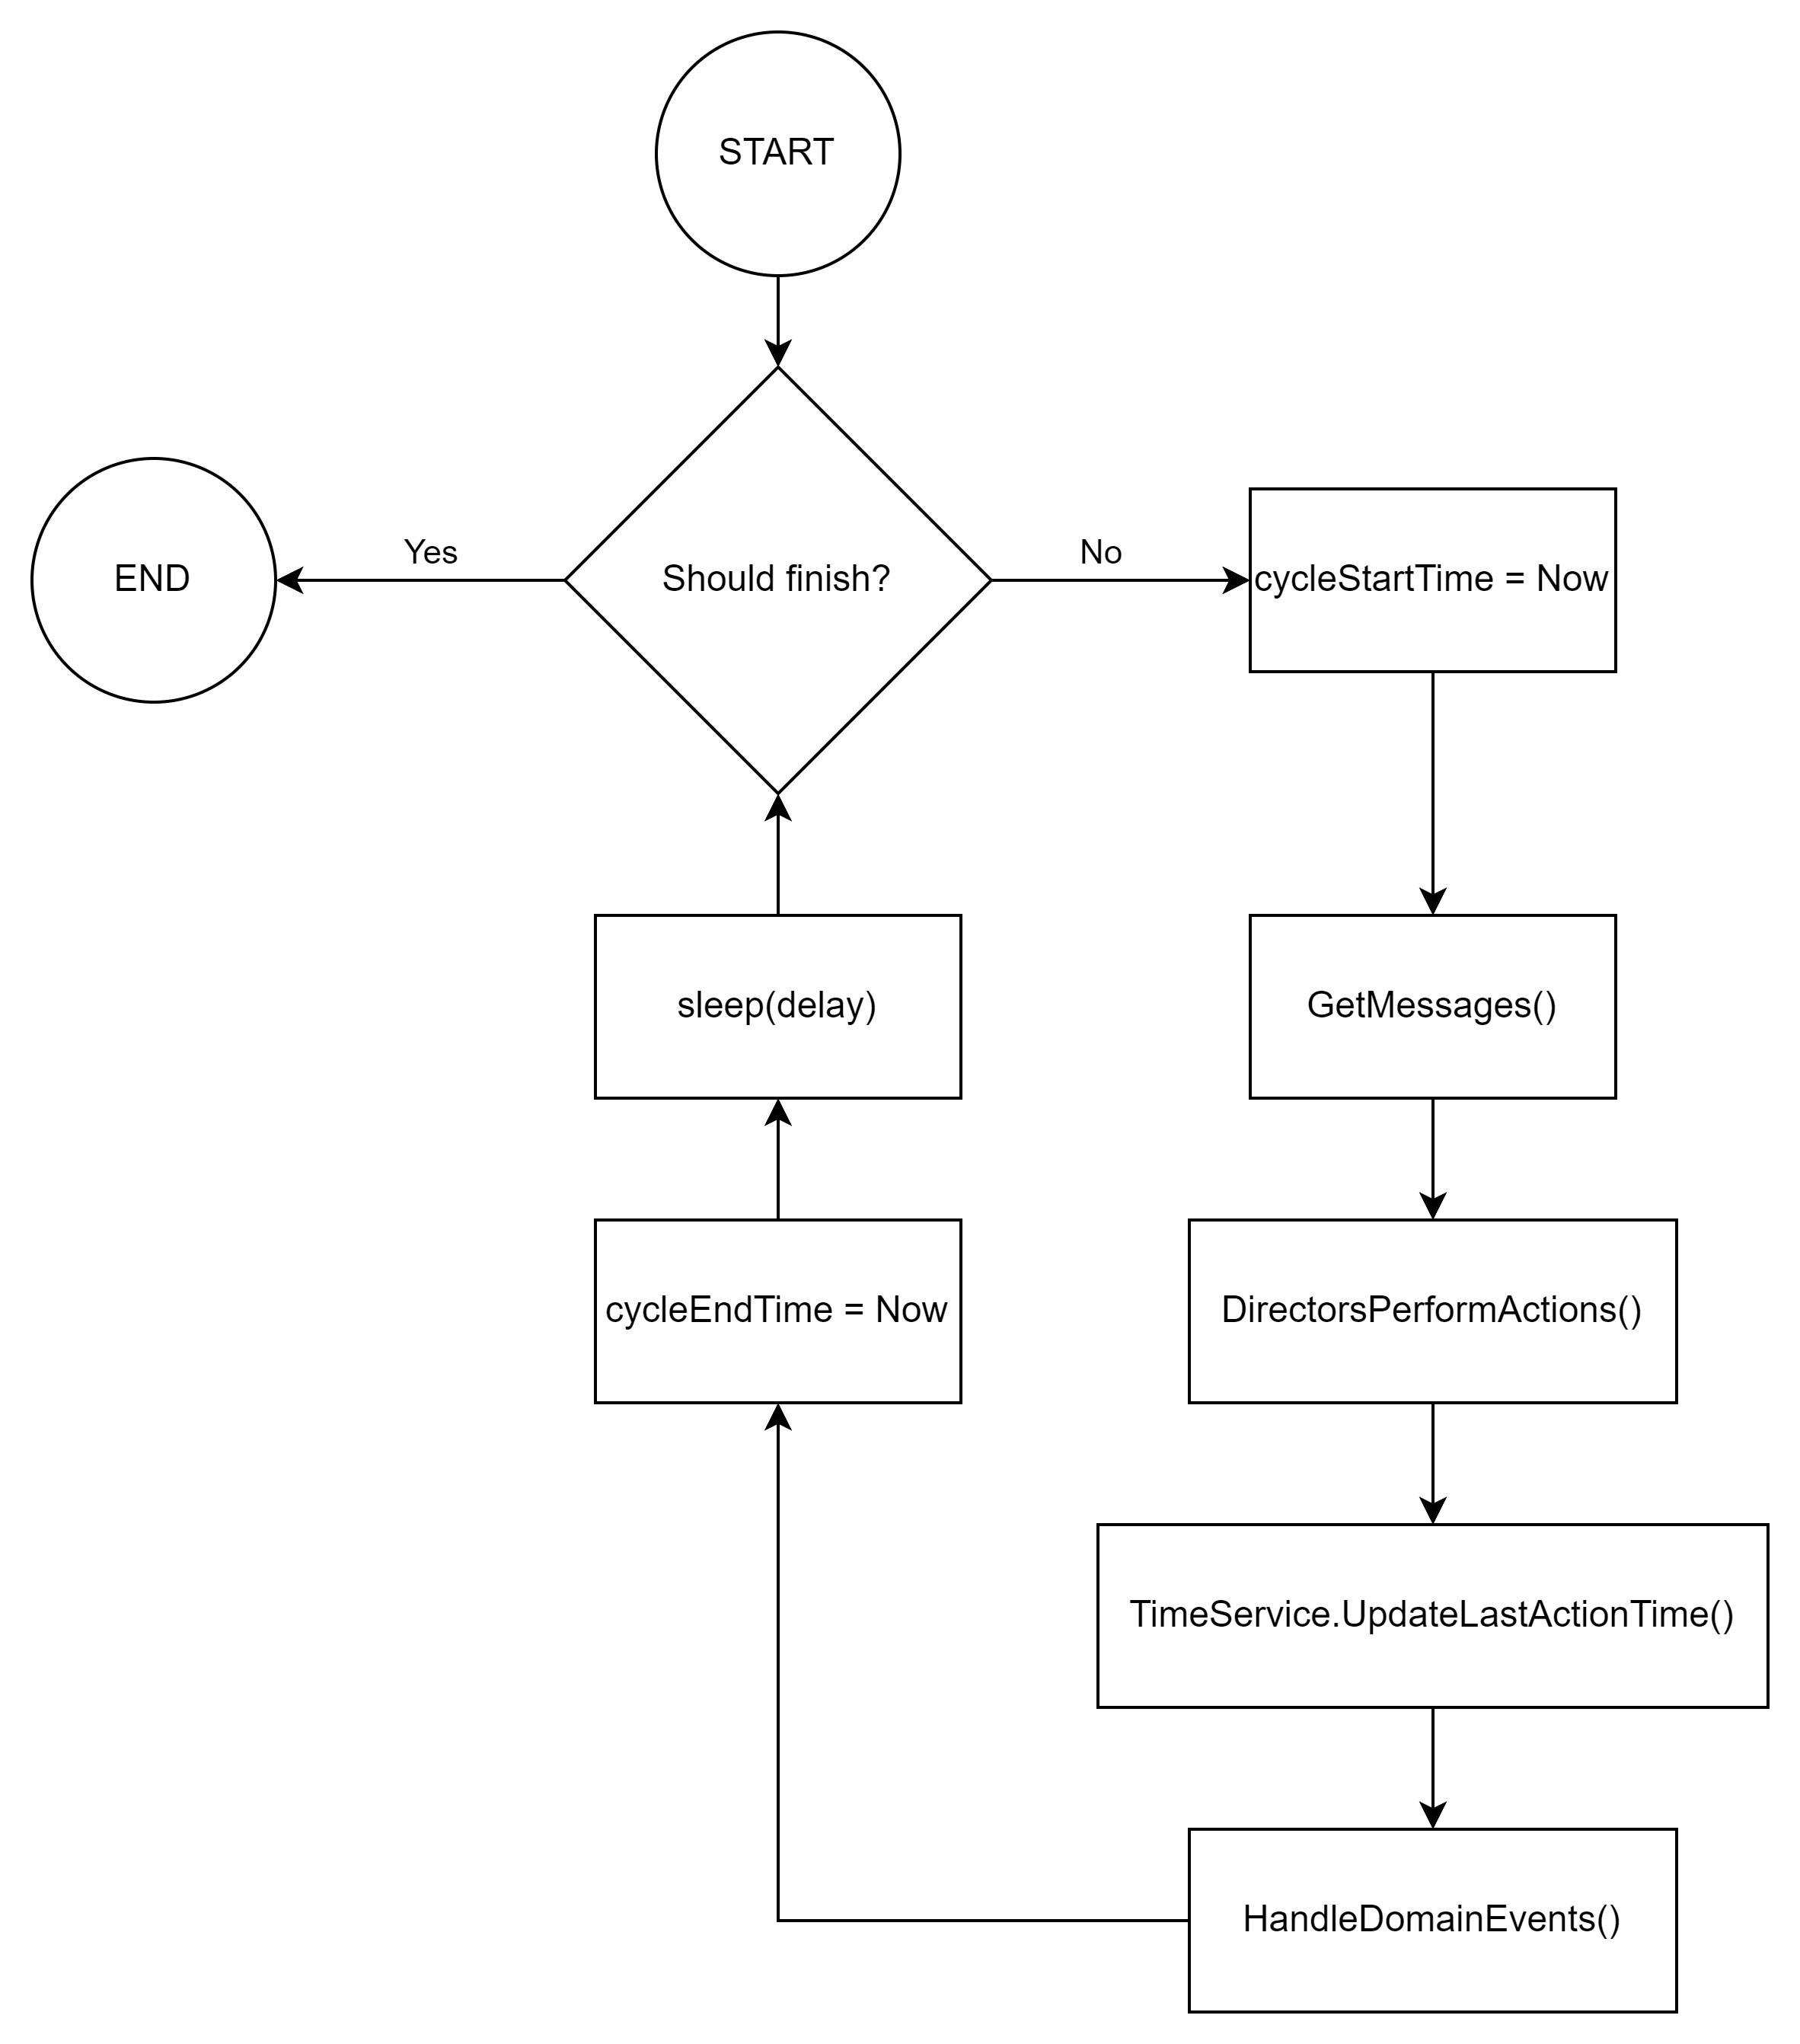
\includegraphics[width=\linewidth]{Simulation - Main Loop}
    \caption{Główna pętla symulacji}
    \label{fig:simulationMainLoop}
    \source{Opracowanie Własne}
\end{figure}

\par Pierwszy z nich odpowiada za generowanie, zarządzanie i przebieg incydentów w mieście. Zgodnie ze swoją konfiguracją, opisaną dokładniej w podrozdziale \ref{sec:konfiguracja}, potrafi tworzyć wydarzenia, jak i pisać ich scenariusze. Po rozpoczęciu danego zdarzenia, oczekuje on na odpowiedź ze strony patrolu, przybycie na miejsce, a następnie przeprowadza przebieg tego wydarzenia, zgodnie z wygenerowanym scenariuszem. Diagram \ref{fig:simulationIncidentLifecycle} przedstawia możliwe zmiany stanów incydentów.

\begin{figure}
    \centering
    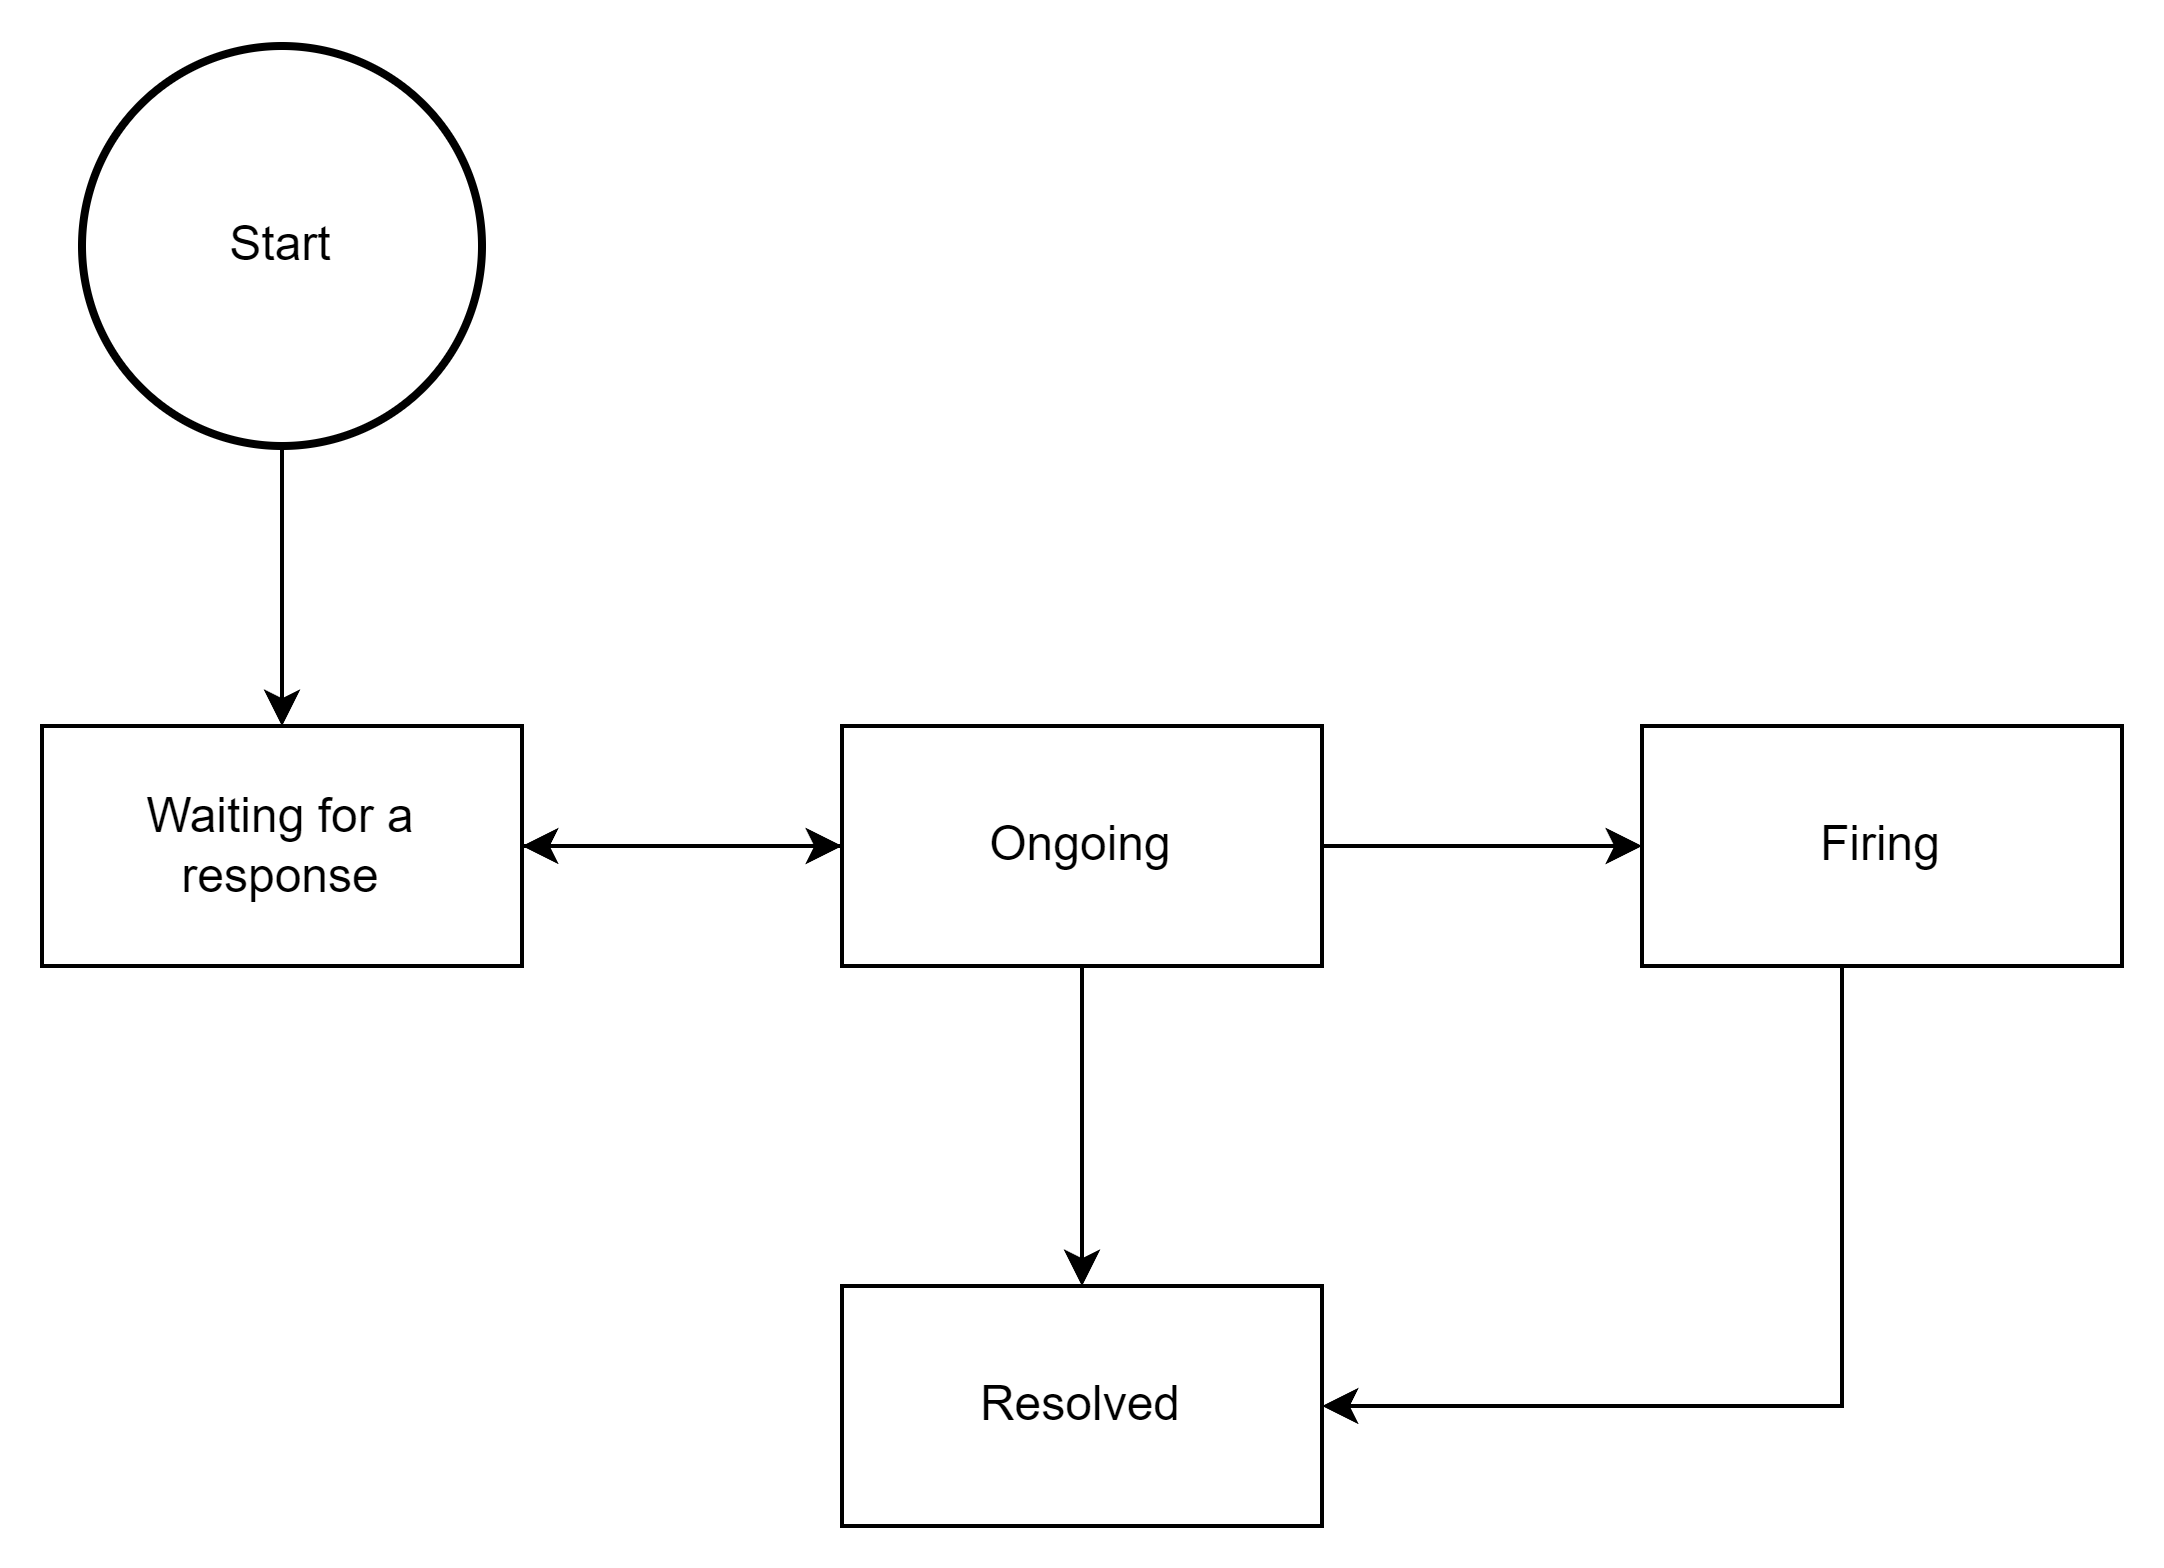
\includegraphics[width=\linewidth]{Incident - Lifecycle}
    \caption{Cykl życia incydentu}
    \label{fig:simulationIncidentLifecycle}
    \source{Opracowanie Własne}
\end{figure}

\par Zadaniem \texttt{PatrolDirector}a jest z kolei zarządzanie jednostkami policji. To on oblicza ich trasy, zarządza obecnie wykonywaną akcją, jak i przemieszcza te jednostki po mieście, według ściśle określonej logiki, która jest w pewnym stopniu konfigurowalna, zgodnie z opisem w podrozdziale \ref{sec:konfiguracja}.

\par Wszystkie zmiany, które zostaną dokonane na obiektach domenowych, automatycznie tworzą w nich tak zwane zdarzenia domenowe\english{Domain Event}. Są one następnie publikowane do zainteresowanych nimi odbiorców. Fragment \texttt{HandleDomainEvents()} przedstawiony na diagramie \ref{fig:simulationMainLoop}.
\section{Konteneryzacja Systemu}
\section{Konfiguracja}
\label{sec:konfiguracja}

\par Zaimplementowane rozwiązanie posiada wiele elementów wymagających skonfigurowania. Od podstawowej konfiguracji działających w nim mikroserwisów, poprzez konfigurację infrastruktury, aż do dostarczenia odpowiednich plików map.

\subsection{Warstwy konfiguracji i ustawiania współdzielone}

\par Ze względu na współdzielenie dużej części kodu pomiędzy wieloma mikroserwisami, również część ich konfiguracji musiała być współdzielona\english{Shared}. Współdzielenie to odbywa się przy wykorzystaniu plików \texttt{sharedsettings.*.json}. Pliki te zawierają ustawienia wykorzystywane przez wszystkie mikroserwisy w systemie. Przykładem takich ustawień może być konfiguracja związana z infrastrukturą. Tabela \ref{tab:configurationSharedSettings} przedstawia wykaz ustawień współdzielonych, wraz z ich znaczeniem.

\begin{table}[H]
    \centering
    \begin{tabular}{|p{0.5\linewidth} | p{0.5\linewidth}|} 
     \hline
     Ustawienie & Znaczenie \\
     \hline
     \hline
     RabbitMq.Host & Host \emph{RabbitMQ} \\ 
     \hline
     RabbitMq.Port & Port \emph{RabbitMQ} \\ 
     \hline
     RabbitMq.Username & Nazwa użytkownika \emph{RabbitMQ} \\ 
     \hline
     RabbitMq.Password & Hasło \emph{RabbitMQ} \\ 
     \hline
     RabbitMq.MessageExchange & Nazwa giełdy dla wiadomości wysyłanych między agentami \\ 
     \hline
     RabbitMq.DirectMessageExchange & Nazwa giełdy dla bezpośrednich wiadomości wysyłanych między agentami \\ 
     \hline
     RabbitMq.EventExchange & Nazwa giełdy dla wydarzeń \\ 
     \hline
     RabbitMq.QueryExchange & Nazwa giełdy dla kwerend \\ 
     \hline
     RabbitMq.CommandExchange & Nazwa giełdy dla komend \\ 
     \hline
     Loki.Uri & URI \emph{Loki}ego \\ 
     \hline
     Loki.Login & Nazwa użytkownika \emph{Loki}ego \\ 
     \hline
     Loki.Password & Hasło \emph{Loki}ego \\ 
     \hline
     SimulationCommunicationSettings.Host & Host \emph{RabbitMQ} dla komunikacji z symulacją \\ 
     \hline
     SimulationCommunicationSettings.Port & Hasło \emph{RabbitMQ} dla komunikacji z symulacją \\ 
     \hline
     SimulationCommunicationSettings.Username & Nazwa użytkownika \emph{RabbitMQ} dla komunikacji z symulacją \\ 
     \hline
     SimulationCommunicationSettings.Password & Hasło \emph{RabbitMQ} dla komunikacji z symulacją \\ 
     \hline
     ServiceSettings.Id & Identyfikator serwisu typu \texttt{GUID} \\ 
     \hline
     ServiceSettings.ServiceType & Typ serwisu. Możliwe wartości: \texttt{HqService}, \texttt{PatrolService}, \texttt{GunService}, \texttt{NavigationService} i \texttt{WebApi}. \\ 
     \hline
    \end{tabular}
    \caption{Wykaz ustawień współdzielonych}
    \label{tab:configurationSharedSettings}
\end{table}

\par Wszystkie te ustawienia mogą jednak zostać nadpisane. Zastosowany został tutaj model warstwowy, gdzie ustawienia z wyższych warstw nadpisują te z niższych. Model warstw przedstawia diagram \ref{fig:configurationLayersModel}. Zaznaczone w nim \texttt{ENVIRONMENT} oznacza zmienną określającą środowisko w jakim aplikacja została uruchomiona. Można ją ustawić za pomocą argumentu \texttt{--environment=ENVIRONMENT} podczas uruchamiania \texttt{dotnet} lub poprzez ustawienie zmiennej środowiskowej \texttt{ASPNETCORE\_ENVIRONMENT} w swoim systemie\cite{MSDOCS_DOTNET_ENVIRONMENTS}.

\par Przykładem zastosowania mechanizmu nadpisywania zmiennych mogą być \texttt{ServiceSettings}. Korzysta z nich każdy serwis działający w aplikacji, jednak są to ustawienia identyfikujące - dlatego znajdują się w \texttt{appsettings.json} konkretnych serwisów.

\par Każde pole konfiguracji może również zostać nadpisane wykorzystując zmienne środowiskowe. Aby uniknąć potencjalnych konfliktów z możliwymi istniejącymi już nazwami, postanowiono dodać \emph{prefix} \texttt{PoliceSupportSystem\_}. Przykładowa nazwa zmiennej środowiskowej powinna wyglądać w następujący sposób: \texttt{PoliceSupportSystem\_ServiceSettings\_\_Id}.

\begin{figure}
    \centering
    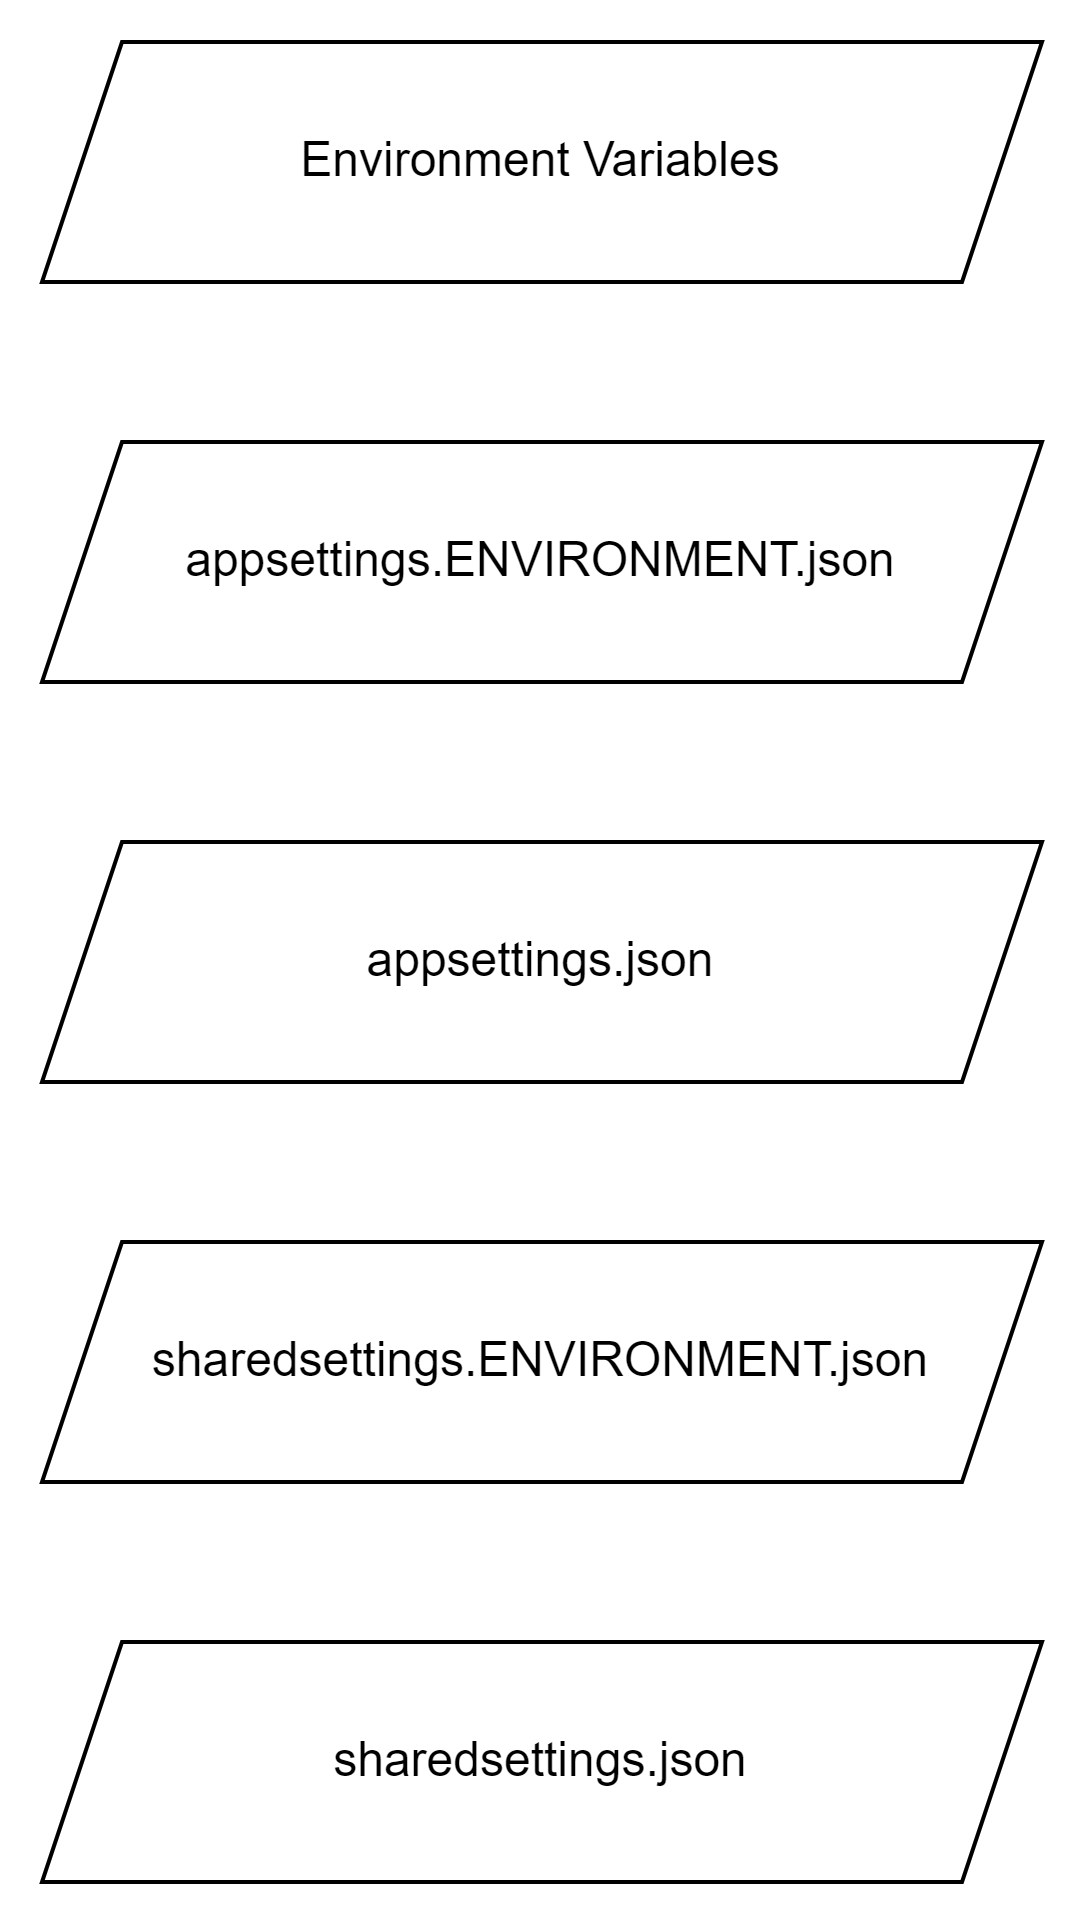
\includegraphics[height=\linewidth]{Configuration - Layers Model}
    \caption{Warstwy konfiguracji}
    \label{fig:configurationLayersModel}
    \source{Opracowanie Własne}
\end{figure}

\subsection{Konfiguracja serwisów i działających w nich agentów}

\par Jedyne ustawienia wymagane do konfiguracji w \emph{Web App} to \texttt{MapSettings}. Zostały one opisane w tabeli \ref{tab:configurationWebAppSettings}.

\begin{table}[H]
    \centering
    \begin{tabular}{|p{0.5\linewidth} | p{0.5\linewidth}|} 
     \hline
     Ustawienie & Znaczenie \\
     \hline
     \hline
     MapSettings.HqLocation.Latitude & Szerokość geograficzna lokalizacji kwatery głównej. Typ: \texttt{double}. \\ 
     \hline
     MapSettings.HqLocation.Longitude & Długość geograficzna lokalizacji kwatery głównej. Typ: \texttt{double}. \\ 
     \hline
    \end{tabular}
    \caption{Ustawienie specyficzne dla \emph{Web App}}
    \label{tab:configurationWebAppSettings}
\end{table}

\par \emph{HQ Service} wymaga skonfigurowania \texttt{HqAgentSettings} i \texttt{DecisionServiceSettings}. Możliwe ustawienia przedstawia tabela \ref{tab:configurationHqServiceSettings}.

\begin{table}[H]
    \centering
    \begin{tabular}{|p{0.5\linewidth} | p{0.5\linewidth}|} 
     \hline
     Ustawienie & Znaczenie \\
     \hline
     \hline
     HqAgentSettings.HqAgentId & Identyfikator \emph{HQ Agent}. Typ: \texttt{GUID}. \\ 
     \hline
     DecisionServiceSettings.EvenPatrolDistribution & Kontroluje przydział patroli do dzielnic. Równomierne lub zależne od \emph{DistrictDangerLevels}. Typ: \texttt{bool}. \\ 
     \hline
     DecisionServiceSettings.DistanceWeight & Waga dla cechy: dystans w algorytmie decyzyjnym. Typ: \texttt{double}. \\ 
     \hline
     DecisionServiceSettings.SameDistrictWeight & Waga dla cechy: patrol w tej samej dzielnicy. Typ: \texttt{double}. \\ 
     \hline
     \makecell[tl]{DecisionServiceSettings\\.InsufficientNumberOfPatrolsInDistrictWeight} & Waga dla cechy: przydział patrolu oddali od wymaganej ilości patroli w dzielnicy, o określonym poziomie niebezpieczeństwa. Typ: \texttt{double}. \\ 
     \hline
     DecisionServiceSettings.DistrictDangerLevels & Słownik zawierający poziomy niebezpieczeństwa dla dzielnic. Typ: \texttt{Dictionary<string, DistrictDangerLevelEnum>}. \\ 
     \hline
     \makecell[tl]{DecisionServiceSettings\\.DangerLevelRequiredPatrollingPatrols} & Ilość wymaganych patroli w zależności od poziomu niebezpieczeństwa dzielnicy. Wpływa na cechę, kontrolowaną przez \texttt{InsufficientNumberOf PatrolsInDistrictWeight}. Typ:\newline \texttt{Dictionary <DistrictDangerLevelEnum,int>}. \\ 
     \hline
    \end{tabular}
    \caption{Ustawienie specyficzne dla \emph{HQ Service}}
    \label{tab:configurationHqServiceSettings}
\end{table}

\par \emph{Patrol Service}, \emph{Navigation Service} i \emph{Gun Service} wymagają skonfigurowania \texttt{PatrolSettings}. Dostępne ustawiania przedstawia tabela \ref{tab:configurationPatrolServiceSettings}.

\begin{table}[H]
    \centering
    \begin{tabular}{|p{0.5\linewidth} | p{0.5\linewidth}|} 
     \hline
     Ustawienie & Znaczenie \\
     \hline
     \hline
     PatrolSettings.PatrolId & Identyfikator patrolu. Typ: \texttt{int}. \\ 
     \hline
     PatrolSettings.PatrolAgentId & Identyfikator \emph{Patrol Agent}. Typ: \texttt{GUID}. \\ 
     \hline
     PatrolSettings.NavigationAgentId & Identyfikator \emph{Navigation Agent}. Typ: \texttt{GUID}. \\ 
     \hline
     PatrolSettings.GunAgentId & Identyfikator \emph{Gun Agent}. Typ: \texttt{GUID}. \\ 
     \hline
    \end{tabular}
    \caption{Ustawienie specyficzne dla patroli}
    \label{tab:configurationPatrolServiceSettings}
\end{table}


\subsection{Konfiguracja symulacji}

\par Jako iż symulacja jest osobną aplikacją i nie posiada żadnych części współdzielonych z pozostałymi serwisami (poza biblioteką \texttt{Simulation.Communication} definiującą wiadomości, które symulacja wysyła i odbiera), to nie wpływają na nią ustawienia z \texttt{sharedsettings.json}. Jedynym źródłem jej konfiguracji, są powiązane z nią pliki \texttt{appsettings.*.json}. Pełen wykaz możliwych ustawień prezentuje tabela \ref{tab:configurationSimulationSettings}.


\begin{longtable}{|p{0.5\linewidth} | p{0.5\linewidth}|} 
     \hline
     Ustawienie & Znaczenie \\
     \hline
     \hline
     SimulationSettings.TimeRate & Definiuje o ile razy szybciej powinien płynąć czas w symulacji, niż w rzeczywistości. Typ: \texttt{double}. \\ 
     \hline
     SimulationSettings.StartDelay & Opóźnienie startu symulacji. Typ: \texttt{TimeSpan?}. \\ 
     \hline
     SimulationSettings.EndAfterSimulationTime & Czas w symulacji, po jakim powinno nastąpić jej zatrzymanie. Typ: \texttt{TimeSpan?}. \\ 
     \hline
     SimulationSettings.HqLocation.Latitude & Szerokość geograficzna lokalizacji kwatery głównej. Typ: \texttt{double}. \\ 
     \hline
     SimulationSettings.HqLocation.Longitude & Długość geograficzna lokalizacji kwatery głównej. Typ: \texttt{double}. \\ 
     \hline
     IncidentDirectorSettings.DistrictDangerLevels & Słownik zawierający konfigurację poziomu niebezpieczeństwa danej dzielnicy. Typ: \texttt{Dictionary<string, DistrictDangerLevelEnum>}, gdzie \texttt{DistrictDangerLevelEnum} może posiadać wartości: \texttt{Low}, \texttt{Normal} i \texttt{High}. \\ 
     \hline
     \makecell[tl]{IncidentDirectorSettings\\.DangerLevelShootingChance.Low} & Szansa na przerodzenie się incydentu w strzelaninę w dzielnicy z \texttt{DistrictDangerLevel} równym \texttt{Low}. Typ: \texttt{double}, wartości $[0, 1]$. \\ 
     \hline
     \makecell[tl]{IncidentDirectorSettings\\.DangerLevelShootingChance.Normal} & Szansa na przerodzenie się incydentu w strzelaninę w dzielnicy z \texttt{DistrictDangerLevel} równym \texttt{Normal}. Typ: \texttt{double}, wartości $[0, 1]$. \\ 
     \hline
     \makecell[tl]{IncidentDirectorSettings\\.DangerLevelShootingChance.High} & Szansa na przerodzenie się incydentu w strzelaninę w dzielnicy z \texttt{DistrictDangerLevel} równym \texttt{High}. Typ: \texttt{double}, wartości $[0, 1]$. \\ 
     \hline
     \makecell[tl]{IncidentDirectorSettings\\.DangerLevelMaxNumberOfIncidentPerDay\\.Low} & Maksymalna ilość incydentów w ciągu dnia dla dzielnicy z \texttt{DistrictDangerLevel} równym \texttt{Low}. Typ: \texttt{int}. \\ 
     \hline
     \makecell[tl]{IncidentDirectorSettings\\.DangerLevelMaxNumberOfIncidentPerDay\\.Normal} & Maksymalna ilość incydentów w ciągu dnia dla dzielnicy z \texttt{DistrictDangerLevel} równym \texttt{Normal}. Typ: \texttt{int}. \\ 
     \hline
     \makecell[tl]{IncidentDirectorSettings\\.DangerLevelMaxNumberOfIncidentPerDay\\.High} & Maksymalna ilość incydentów w ciągu dnia dla dzielnicy z \texttt{DistrictDangerLevel} równym \texttt{High}. Typ: \texttt{int}. \\ 
     \hline
     PatrolDirectorSettings.NormalPatrolSpeed & Prędkość patrolu wyrażona w $km/h$ w warunkach normalnych. Typ: \texttt{double}. \\ 
     \hline
     PatrolDirectorSettings.EmergencyPatrolSpeed & Prędkość patrolu wyrażona w $km/h$ w warunkach specjalnych. Typ: \texttt{double}. \\ 
     \hline 
     RabbitMqSettings.Host & Host \emph{RabbitMQ} \\ 
     \hline 
     RabbitMqSettings.Port & Port \emph{RabbitMQ} \\ 
     \hline 
     RabbitMqSettings.Username & Nazwa użytkownika \emph{RabbitMQ} \\ 
     \hline 
     RabbitMqSettings.Password & Hasło \emph{RabbitMQ} \\ 
     \hline 
     LokiSettings.Uri & URI \emph{Loki}ego \\ 
     \hline 
     LokiSettings.Login & Nazwa użytkownika \emph{Loki}ego \\ 
     \hline
     LokiSettings.Password & Hasło \emph{Loki}ego \\ 
     \hline
     DbSettings.Host & Host \emph{PostgreSQL} \\ 
     \hline
     DbSettings.Port & Port \emph{PostgreSQL} \\ 
     \hline
     DbSettings.Username & Nazwa użytkownika \emph{PostgreSQL} \\ 
     \hline
     DbSettings.Password & Hasło \emph{PostgreSQL} \\ 
     \hline
     DbSettings.DbName & Nazwa bazy danych \emph{PostgreSQL} zawierającej zaimportowane dane. \\ 
     \hline
\caption{Wykaz ustawień symulacji}
\label{tab:configurationSimulationSettings}
\end{longtable}


\subsection{Docker}

\par Konfiguracja niektórych serwisów odbywa się w plikach \emph{Docker Compose}\cite{DOCKER_COMPOSE_DOCS}. W tym celu korzysta się z możliwości ustawienia zmiennych środowiskowych dla danego kontenera. Jest to sekcja \texttt{environment} danego pliku \emph{compose}.

\par Import map odbywa się na bazie konfiguracji w pliku \texttt{infrastructure-docker-compose.yaml}. Aby poprawnie zaimportować przygotowane pliki map, musimy w je wskazać w zmiennych środowiskowych \texttt{MAP\_FILE} i \texttt{DISTRICTS\_FILE} oraz umieścić w folderze \texttt{./SimulationDb/maps}.

\par Mechanizm ten jest również wykorzystywany przy konfiguracji patroli, biorących udział w działaniu systemu. Aby dodać patrol należy go zdefiniować w pliku \texttt{docker-compose.yaml}. Konfiguracja ta wykorzystuje zmienne środowiskowe, aby ustawić odpowiednie identyfikatory serwisom patrolu. Zostało to dokładniej opisane w podrozdziale \ref{sec:konteneryzacjaSystemu}.


\chapter{Metodologia i analiza wyników badań}
\section{Problem badawczy}
\label{sec:problemBadawczy}

\par Zaprojektowany system pozwala śledzić i symulować działania jednostek policji w inteligentnym mieście. Głównym celem jest zbadanie, jak w efektywny sposób można zarządzać tymi jednostkami. Sprawdzenie wpływu kontekstu podczas ich rozmieszczania, jak i w trakcie wydawania poleceń.

\par System posiada wiele zmiennych, które umożliwiają jego konfigurację w zależności od potrzeb. Istotnym jest jednak wybranie konkretnych cech, którymi chcemy manipulować, aby otrzymać pełen obraz jego działania.

\par Aby dobrze ocenić otrzymane rezultaty, koniecznym jest wybranie cech, które zostaną porównane. Więcej na ten temat zostało opisane w podrozdziale \ref{sec:wyborMetodyBadawczejIUzasadnienie}.
\section{Wybór metody badawczej i uzasadnienie}
\label{sec:wyborMetodyBadawczejIUzasadnienie}

\par Do oceny wyników zostanie zastosowanie porównanie wybranych wskaźników, obliczonych na podstawia analizy danych wyeksportowanych z systemów. Wybrane wskaźniki to:
\begin{itemize}
    \item średnia odległość rozważanego patrolu od miejsca incydentu w trakcie podejmowania decyzji,
    \item średnia odległość wybranego patrolu od miejsca incydentu w trakcie podejmowania decyzji,
    \item średni czas potrzebny na dotarcie do miejsca zdarzenia,
    \item ilość aktywnych incydentów w czasie.
\end{itemize}
Wskazują one efektywność w rozwiązywaniu incydentów. Szczególnie istotnym jest tutaj wskaźnik ilości aktywnych incydentów w czasie. Ponieważ jeżeli ich ilość ciągle się zwiększa, oznacza to, że system nie jest w stanie odpowiednio szybko ich rozwiązywać.

\par Aby prawidłowo ocenić wpływ danych kontekstowych na algorytm decyzyjny, tylko one, a konkretniej wagi im przypisane, podlegają manipulacji. Zmienne podlegające eksperymentom, zostały przedstawione w tabeli \ref{tab:zmiennePodlegająceEksperymentom}. Pozostałe ustawienia są stałe i zostały one przedstawione w tabelach \ref{tab:ustawieniaSymulacji} i \ref{tab:ustawieniaHqService}.

\begin{table}[H]
    \centering
    \begin{tabular}{|c|}
        \hline
        Nazwa zmiennej \\
        \hline
        \hline
         \texttt{EvenPatrolDistribution} \\
         \hline
         \texttt{DistanceWeight} \\
         \hline
         \texttt{SameDistrictWeight} \\
         \hline
         \texttt{InsufficientNumberOfPatrolsInDistrictWeight} \\
         \hline
    \end{tabular}
    \caption{Zmienne podlegające eksperymentom}
    \label{tab:zmiennePodlegająceEksperymentom}
\end{table}

\begin{longtable}{|p{0.5\linewidth} | p{0.5\linewidth}|} 
    \hline
     Ustawienie & Wartość \\
     \hline
     \hline
     \makecell[tl]{SimulationSettings.TimeRate} & 240 \\
     \hline
     \makecell[tl]{SimulationSettings.EndAfterSimulationTime} & 1.00:00:00 \\
     \hline
     \makecell[tl]{IncidentDirectorSettings\\.DangerLevelShootingChance\\.Low} & 0 \\
     \hline
     \makecell[tl]{IncidentDirectorSettings\\.DangerLevelShootingChance\\.Normal} & 0.02 \\
     \hline
     \makecell[tl]{IncidentDirectorSettings\\.DangerLevelShootingChance\\.High} & 0.1 \\
     \hline
     \makecell[tl]{IncidentDirectorSettings\\.DangerLevelMaxNumberOfIncidentPerDay\\.Low} & 5 \\
     \hline
     \makecell[tl]{IncidentDirectorSettings\\.DangerLevelMaxNumberOfIncidentPerDay\\.Normal} & 15 \\
     \hline
     \makecell[tl]{IncidentDirectorSettings\\.DangerLevelMaxNumberOfIncidentPerDay\\.High} & 30 \\
     \hline
     \makecell[tl]{PatrolDirectorSettings\\.NormalPatrolSpeed} & 50 \\
     \hline
     \makecell[tl]{PatrolDirectorSettings\\.EmergencyPatrolSpeed} & 80 \\
     \hline
\caption{Ustawienia symulacji}
\label{tab:ustawieniaSymulacji}
\end{longtable}

\begin{longtable}{|p{0.5\linewidth} | p{0.5\linewidth}|} 
    \hline
    Ustawienie & Wartość \\
    \hline
    \hline
    \makecell[tl]{DecisionServiceSettings\\.DangerLevelRequiredPatrollingPatrols\\.Low} & 0 \\
    \hline
    \makecell[tl]{DecisionServiceSettings\\.DangerLevelRequiredPatrollingPatrols\\.Normal} & 1 \\
    \hline
    \makecell[tl]{DecisionServiceSettings\\.DangerLevelRequiredPatrollingPatrols\\.High} & 2 \\
    \hline
    Ilość patroli & 20 \\
    \hline
\caption{Ustawienia stałe \emph{HQ Service}, \emph{HQ Agent} oraz patroli}
\label{tab:ustawieniaHqService}
\end{longtable}

\par Mapa Krakowa została wybrana, jako miejsce do przeprowadzenia eksperymentów. Dzielnicom zostały przydzielone poziomy niebezpieczeństwa. Są one przedstawione na grafice \ref{fig:districtDangerLevelMap}.

\begin{figure}
    \centering
    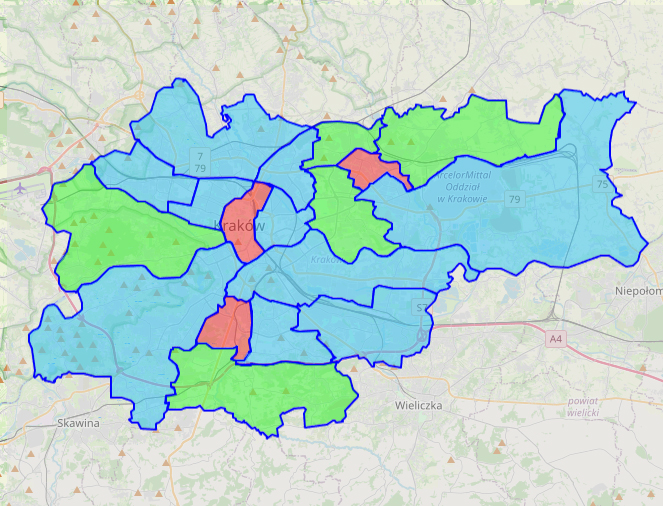
\includegraphics[width=\linewidth]{Districts - Danger Level Map}
    \caption{Kraków - dzielnice i ich poziomy niebezpieczeństwa. Zielony - \emph{Low}, Niebieski - \emph{Normal}, Czerwony - \emph{High}.}
    \label{fig:districtDangerLevelMap}
    \source{Opracowanie Własne}
\end{figure}

\par Aby zdobyć wiarygodną próbkę danych, każdą z konfiguracji postanowiono uruchomić trzykrotnie, a następnie obliczyć średnią z uzyskanych wyników. Decyzja ta została podjęta, aby ograniczyć błąd wynikający z niedeterministycznej natury symulacji.
\section{Uzyskane wyniki i ich analiza}
\chapter{Podsumowanie i wnioski}

\par Aby spełnić założenia projektu, została przeprowadzona analiza systemów agentowych, systemów rozproszonych, komunikacji w ramach systemów rozproszonych, jak i wykorzystania map \emph{OSM}. Zbadane zostały również dane kontekstowe, pojawiające się w systemie w odniesieniu do obcujących z nimi agentów. Dane te zostały skategoryzowane, jak i została pokazana ich rola w systemie.

\par W ramach tej pracy, został zaimplementowany rozproszony system mikroserwisowy, z serwisami, w których działają agenci. Dodatkowo została również zaimplementowana symulacja, pozwalająca na przetestowanie działania systemu i przeprowadzenie na nim eksperymentów. Powstała również aplikacja \emph{web}owa, umożliwiająca wizualizację i agregacją danych, dotyczących przebiegu działania. Całość powstałego rozwiązania łączy się za pomocą \emph{RabbitMQ}. Elementy systemu zostały zintegrowane z \emph{PostGIS}, \emph{pgRouting} i \emph{Grafana Loki}. Sumarycznie, powstała implementacja zawiera ponad $20000$ linijek kodu.

\par Dodatkowo, system został skonteneryzowany, wykorzystując technologię \emph{Docker}. Dzięki temu możliwym jest skalowanie systemu, w przypadku chęci przeprowadzenie eksperymentów, z wykorzystaniem jego bardziej złożonej wersji, w której bierze udział więcej agentów.

\par Stworzony system jest wrażliwy na dane kontekstowe. Informacje te, są wykorzystywane przez agentów, którzy postrzegają i wpływają na swoje otocznie. Jak wykazała analiza, kontekst może pełnić istotną rolę w procesie decyzyjnym i odpowiednia jego interpretacja, może wpłynąć pozytywnie na rezultaty działania systemu. Pozwala on na podjęcie rozsądniejszej decyzji, która przynosi efektywne rezultaty. Nie należy jednak zapominać, że otrzymane wyniki dotyczą ściśle określonej konfiguracji. Powstały system jest jednak narzędziem, pozwalającym na dalsze badania tej dziedziny.

% itd.
\appendix
% \include{appendageA}
% \include{dodatekB}
% itd.

\printbibliography

\end{document}